% !TEX encoding = UTF-8
% !TEX TS-program = pdflatex
% !TEX root = ../Relazione.tex
% !TEX spellcheck = it-IT
\clearpage
%%%%%%%%%%%%%%%%%%%%%%%
\section{Network breakdown}
\label{sec:attaack}
%%%%%%%%%%%%%%%%%%%%%%%
%(formerly "Analisi percolativa" ma questo è un titolo noioso, meglio una roba più deep impact ogliea) 

Una volta osservate le distribuzioni del grado nelle reti delle quattro compagnie e nella rete complessiva formata da tutte le antenne comprese nell'area metropolitana di Roma, procediamo con lo studio percolativo. Si è scelto di simulare due differenti scenari in cui i nodi della rete vengono disabilitati \textcite{Barbalbert2000}. Nel primo scenario si è ipotizzato un attacco intenzionale che cominciasse dai nodi con maggior grado, nel secondo una rimozione random.

Lo scopo è studiare l'andamento, in funzione della percentuale di nodi rimossi, del diametro $D$ della rete e della dimensione del cluster più grande (verificando che esso sia il Giant Cluster della rete) rapportata al numero totale di nodi sopravvissuti. A seconda di come la rete si comporterà, sarà possibile dedurne la robustezza nei due scenari, in modo tale da poter confrontare meglio tale comportamento con quello di una rete scale-free o random di pari grado medio $\langle k \rangle$.

In tutti e cinque i campioni di rete che abbiamo analizzato, sono stati conteggiati gli andamenti di alcune grandezze topologiche e statistiche di interesse: oltre a dimensione del giant cluster, $D$, anche $\langle l \rangle$, coefficiente di clustering globale $C$, $\langle k \rangle$ e $\langle k^2 \rangle/\langle k \rangle$. I grafici ottenuti sono stati messi a confronto a quelli ottenuti con le reti generate secondo i modelli.

È importante ricordare che la rete reale ha ovviamente delle contromisure per evitare la caduta delle comunicazioni. Le antenne trasmettono segnali tra loro su due bande di frequenza: una \emph{user-side}, dedicata alle normali trasmissioni tra utenti del servizio, e una dedicata a un complesso sistema di feedback gestito da degli \emph{hub}(grosse antenne con raggio sui $20\:km$). Questa struttura gerarchica permette, nel caso di caduta di una antenna o di un improvviso eccessivo carico in una zona circoscritta, che gli hub gestiscano potenza e capacità delle antenne circostanti mentre vengono inviati tecnici per un intervento sul luogo.

Questo sistema ha un certo tempo di reazione. L'analisi da noi svolta pertanto suppone che la caduta della rete avvenga in un tempo inferiore, in una sorta di approssimazione adiabatica. Inoltre, la sola caduta degli hub sarebbe già sufficiente a compromettere seriamente l'integrità della rete (le antenne avrebbero difficoltà a coordinare le comunicazioni tra loro), ma nella nostra ipotesi di mesh-network distribuita ci interessano soltanto le comunicazioni nelle frequenze user-side. Usando questo modello semplificato siamo riusciti a ottenere alcune informazioni su una ipotetica rete cittadina di questa natura.

\subsection{Speedup del codice (parte 1: multiprocessing)}

Per le simulazioni di attacco intenzionale e random failure sulle reti in esame e lo studio approfondito dell'andamento delle grandezze statistiche e topologiche durante l'analisi percolativa, abbiamo inizialmente utilizzato \emph{networkx}, una libreria di Python piuttosto completa dedicata alle reti.

Tuttavia questa si è rivelata una scelta sbagliata, in quanto networkx, pur essendo molto completa e semplice da usare, non è particolarmente ottimizzata dal punto di vista dell'efficienza di calcolo. Questo perché è interamentente scritta in Python, anche per le sue routine più interne e non implementa alcun tipo di parallelismo built-in.

Creare, manipolare e disegnare i grafi sono operazioni semplici e immediate, ma ma quando si cercano di usare le funzioni più pesanti dal punto di vista del calcolo, come per esempio quella per determinare il diametro della rete, networkx appare del tutto non soddisfacente.

Per esempio, il calcolo di diametro, average path lenght, coefficiente di clustering e dimensioni del giant cluster impiegava 20 secondi per una singola iterazione con la rete Tre (la più piccola, circa 1400 nodi), 50 secondi per Tim e Vodafone (circa 1800 nodi entrambe) mentre con la rete Wind (la più grande, con circa 2350 nodi) impiegava ben 2.5 minuti. Questo dato, moltiplicato per i 100 passi richiesti, porta ad una previsione di più di 6 ore di calcolo per l'analisi percolativa di tutte le singole reti.

Abbiamo osservato che i tempi scalano all'incirca quadraticamente con il numero di nodi, per cui per lo studio della rete complessiva di tutta Roma sarebbero richiesti 20 minuti per una iterazione e quasi 30 ore di calcolo per l'analisi completa. Queste considerazioni rendevano di fatto impraticabile questa strada.

\begin{figure}[ht!]
	\centering
	
\includegraphics[width=0.55\textwidth]{./Immagini/Attack/meme_Leonida.jpg}
\end{figure}

Dato che i tempi di calcolo richiesti per l'analisi percolativa risultavano spropositati, soprattutto nel caso di random failure, abbiamo cercato dei modi per velocizzare il calcolo ed aggirare il problema.

In primis si è cercato di evitare operazioni cicliche sui vettori dinamici, come \lstinline{pop()} e \lstinline{append()} e di utilizzare sempre librerie python ottimizzate e internamente scritte in C, come ad esempio \emph{numpy}. Già questo permette operazioni su grossi vettori con un incremento di prestazioni rispetto al python puro di almeno il doppio.

Inoltre si è tentato di sfruttare i diversi core della macchina, facendo degli esperimenti di rudimentale calcolo parallelo. In pratica si è cercato di rendere il codice non sequenziale, in modo da usare funzioni del tutto indipendenti e poter scrivere tutto quanto in termini di funzioni \lstinline{map()} per poi utilizzare la libreria built-in \emph{multiprocessing} e fare una prima parallelizzazione. 

\begin{lstlisting}
import multiprocessing
cpus = multiprocessing.cpu_count()
pool = multiprocessing.Pool(processes=cpus)
pool.map(function, array)
\end{lstlisting}

Abbandonare il paradigma sequenziale rendendo le funzioni totalmente indipendenti tra loro fa sì che esse possano girare in contemporarea riducendo il tempo di calcolo, ma nel contempo aumenta il quantitativo di RAM richiesta dal programma, quasi dello stesso fattore. Pertanto bisogna fare attenzione a far girare il programma su una macchina adeguata sotto tutti i punti di vista.

Purtroppo peò nel nostro caso questo approccio non si è rivelato adatto. Nel fare i tentativi vedevamo che i processori lavoravano insieme al 100\% per un primo periodo, per poi ibernarsi in una eterna fase di stallo al 20\% del carico, probabilmente per incongruenze nel messaging tra le varie istanze di python. Non possedendo sufficienti conoscenze su calcolo parallelo e cloud computing per poter risolvere velocemente il problema, abbiamo dunque abbandonato questo aproccio.

\begin{figure}[h!]
	\centering
	
\includegraphics[width=0.55\textwidth]{./Immagini/Attack/meme_Boromir.jpg}
\end{figure}

\subsection{Strategie di attacco}
\label{subsec:atakstrat}
L'esigenza di provare a parallelizzare il codice ci ha portato a due versioni differenti della funzione di attacco intenzionale: una sequenziale e una parallela. Entrambe le varianti rimuovono circa l'1\% dei nodi per volta: 

\begin{itemize}
 \item La funzione sequenziale elimina l'insieme dell'1\% dei nodi più importanti, analizza la rete e calcola il prossimo insieme di 1\% di nodi da rimuove.
 \item La funzione parallela ha invece un comportamento più adiabatico: guarda il grafo iniziale e fa una classifica assoluta dei nodi per importanza, rimuovendone di volta in volta l'1\% in maniera ordinata.
\end{itemize}

Possiamo supporre che un reale attacco alla rete sia portato avanti con modalità adiabatiche: un ipotetico terrorista piazza nella notte delle cariche esplosive sotto le antenne che ritiene fondamentali e poi le fa scoppiare in un secondo momento tutte in una volta. A titolo di esempio, possiamo immaginare che l'attacco si consideri riuscito quando metà dell'area metropolitana rimane isolata senza possibilità di comunicare. Questo è il parametro finale in base al quale viene scelta la sequenza di antenne da far esplodere.

Ma chi garantisce che questa sequenza coincide con gli N nodi di grado maggior all'istante iniziale? In altre parole: è questa una strategia \emph{ottimale}?\\
La risposta è no! La strategia ottimale è quella che, a parità di risultato, coinvolge il minor numero di antenne fatte eplodere, anche per minimizzare il rischio di essere scoperto nella notte mentre piazza l'esplosivo in giro per la città.

\begin{figure}[t!]
	\centering
	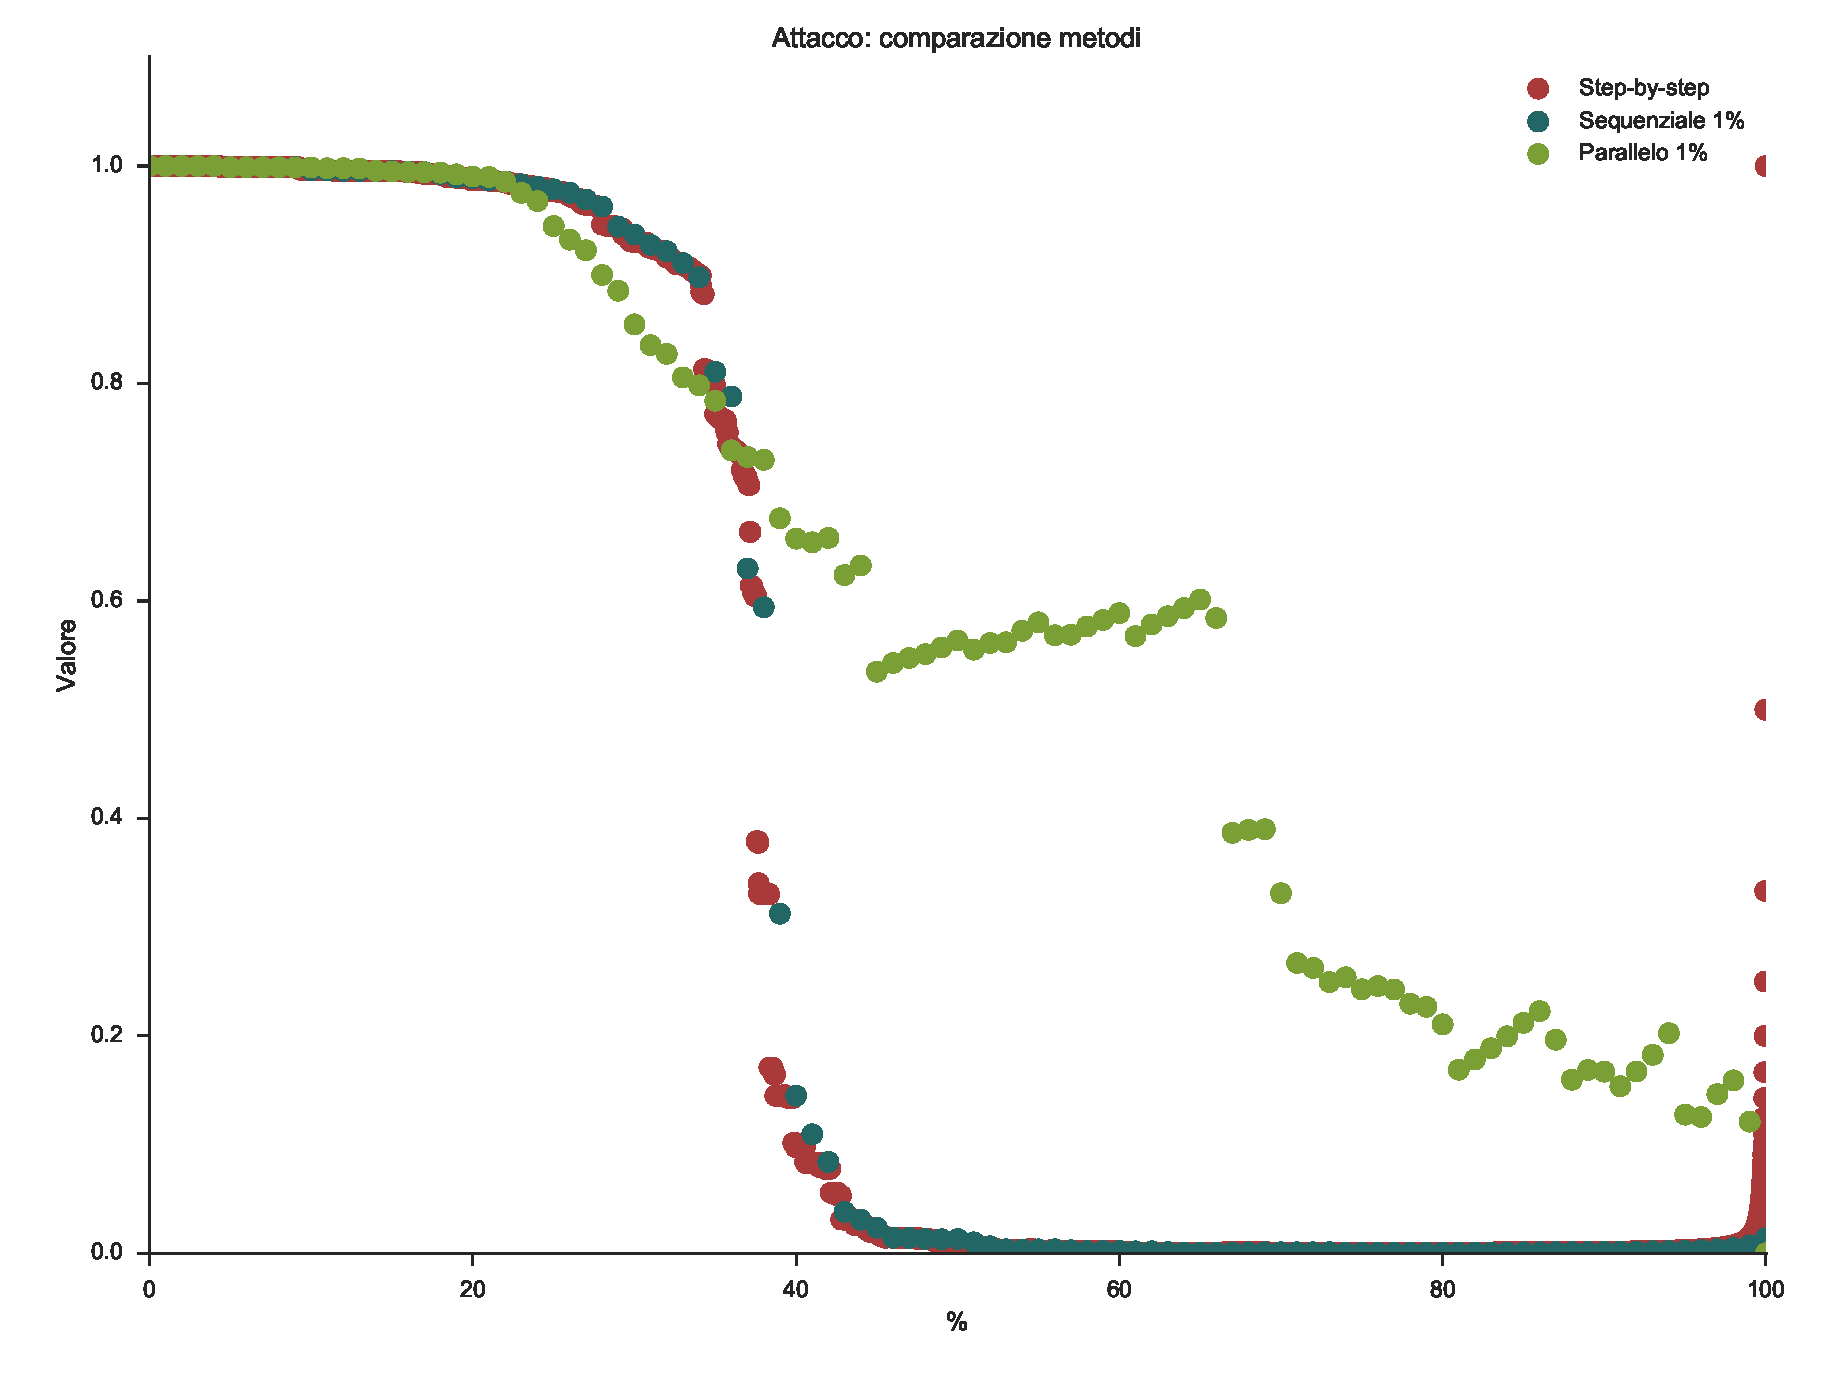
\includegraphics[width=0.65\textwidth]{./Immagini/Attack/AttackGC_Compare}
	\caption[Confronto metodi.]{Confronto sugli effetti dei tre metodi di attacco sulla dimensione del giant cluster.}
	\label{fig:compattack}
\end{figure}

Tale strategia può essere evidenziata solo da una simulazione \textbf{sequenziale}, attuata facendo evolvere la rete passo per passo, secondo una strategia di \emph{steepest descent}. Questo garantisce di trovare la strategia ottimale, soprattutto se vengono inclusi anche gli effetti a cascata dovuti all'overload e alla saturazione di banda. Dal grafico sottostante (attacco intenzionale) si evince comunque che non c'è molta differenza tra procedere sequenzialmente con un campionamento all'1\% o eseguire una simulazione di attacco nodo per nodo, per cui ad ogni modo il costo computazionale complessivo non risulta eccessivo.

Nel caso di random failure (escludendo gli effetti di saturazione a cascata) non c'è invece alcuna differenza tra l'approccio sequenziale e quello \textbf{parallelo}, rendendo il secondo algorimo preferibile nel caso si voglia sfruttare tutta la potenza delle moderne CPU \emph{multicore}.

Riassumendo: 
\begin{itemize}
 \item Nel caso di intentional attack è doveroso usare un approccio sequenziale. 
 \item Nel caso di random failure è consigliabile utilizzare un approccio parallelo.
\end{itemize}

\subsection{Speedup del codice (parte 2: graph-tool)}
Come già detto la prima soluzione al problema dei tempi è stata tentare una parallelizzazione del codice in python: dato che networkx non supporta il calcolo parallelo interno, si è tentato di parallelizzare le funzioni di attacco intenzionale e random failure. Abbiamo però mostrato come alcuni degli algoritmi siano intrinsecamente sequenziali.

Un possibile metodo per ovviare a ciò sarebbe potuto essere generare e salvare in memoria tutte le reti a tutte le iterazioni e successivamente usare delle funzioni parallelizzabili per l'analisi. Tuttavia con networkx la richiesta di tempo di calcolo rimane comunque alta e si aggiungerebbe anche il problema della memoria RAM, dello spazio su disco e dei tempi di lettura e scrittura.

L'unica via praticabile è stata ripiegare su \emph{graph-tool}: un'altra libreria meno \emph{user-friendly} ma estremamente più efficiente e sopratutto impostata di default sul calcolo parallelo. Le funzioni di analisi topologica e statistica sono molto più veloci rispetto a networkx, poiché implementate in C con il \emph{template programming} ed ottimizzate in fase di compilazione. Inoltre la possibilità di usarle nativamente in parallelo su 4 core e 8 thread ci ha permesso di calcolare le singole funzioni con una velocità più di 60 volte superiore a prima.

Considerato ciò, il codice per lo studio percolativo delle reti è stato convertito (con non poco sforzo) per poter fare uso della nuova libreria. Alla fine, per l'analisi percolativa completa di tutte le reti, ovvero con lo studio, in funzione dei nodi rimossi, delle quantità 

\begin{itemize}
 \item   diametro $D$
 \item   average path lenght $\langle l \rangle$
 \item   clustering coefficient $C$
 \item   average degree $\langle k \rangle$
 \item   dimensioni del giant cluster
 \item   criterio di soglia percolativa (andamento di $\langle k^2 \rangle / \langle k \rangle$)
\end{itemize}

da una previsione iniziale di più di 24 ore di tempo di calcolo si è passati a circa $3/4$ d'ora, con uno speedup di circa un fattore 30.

\begin{figure}[h!]
	\centering
	
\includegraphics[width=0.55\textwidth]{./Immagini/Attack/meme_Obama.jpg}
\end{figure}

\subsection{Random failure}
Le reti da cui è partito lo studio percolativo sono le 5 definite e costruite nel precedente paragrafo. Le grandezze iniziali erano:


\begin{table}[ht!]
\centering
% \caption{Dati iniziali delle reti studiate.}
	\begin{tabular}{cccccccccc}
	\toprule
	Rete		&N		&$GC\%$	&$D$	&$\langle l\rangle$	&$C$		&$\langle k\rangle$	&$C/\langle k\rangle$	&$\langle k^2\rangle/\langle k\rangle$	&$f\%$\\
	\midrule  
	Tim		&1756	&1		&2	&1.96			&0.89	&64.3			&0.014				&359							&99.7\\
	Vodafone	&1771	&1		&2	&1.97			&0.87	&52.9			&0.016				&243							&99.6\\
	Wind		&2365	&1		&2	&1.96			&0.89	&97.3			&0.009				&478							&99.8\\
	Tre		&1395	&1		&2	&1.97			&0.88	&41.4			&0.021				&239							&99.6\\
	Roma		&7287	&1		&2	&1.97			&0.89	&239.1			&0.004				&1353							&99.9\\
	\bottomrule
	\end{tabular}
\caption{Grandezze topologiche e statistiche delle reti a $t=0$}
\label{tab:datiInitial}
\end{table}

La prima cosa da notare è che le reti delle singole compagnie hanno un rapporto coefficiente di clustering-grado medio in linea con molte altre reti reali \parencite{Barbalbert2002}, e che la rete costruita con tutte le antenne non vede aumentare particolarmente il suo clustering. Inoltre ci si aspetta che le reti siano tutte particolarmente resistenti sotto random failure, comportamento che sembra più simile a quello di una rete scale free. Tuttavia una rete random con un grado medio alto ha comunque un $f$ molto alto. Per esempio, una rete random avente $N = N_{Tim}$ e $\langle k \rangle = \langle k \rangle_{Tim}$, avrebbe una $f$ critica di poco inferiore: $\sim 98\%$. Infatti, essendo per una rete random $\langle k \rangle = Np$, perché sia uguale a $\langle k \rangle_{Tim}$ con $\sim 1800$ nodi, deve essere $p \sim 3.7\%$, 
$$\Rightarrow \sigma^2 = Np(1-p) = \langle k^2 \rangle - \langle k \rangle^2 \sim 62$$
$$\Rightarrow \frac{\langle k^2 \rangle }{\langle k \rangle} = \frac{Np(1-p)-(Np)^2}{Np} \sim 1+Np = 1+ \langle k \rangle \sim 65$$
$$\Rightarrow f \sim 1 - \frac{1}{65} \sim 98\%$$

Con una rete random costruita con i parametri della rete totale si ottiene $f = 99.5$. Valori quindi che si distinguono poco dalla soglia per una rete power-law finita, anche nel caso in cui l'esponente sia di poco maggiore di 3: $f \sim 1 - \frac{1}{\frac{\gamma - 2}{\gamma-3}k_{max}} > 90\%$ già per un grado massimo di $\sim10$.


\subsubsection{Attacco intenzionale}
Nello scenario di attacco intenzionale ci si aspetta una veloce frammentazione della rete. I cluster diverranno rapidamente più piccoli fino a frammentarsi del tutto entro pochi punti percentuali di nodi rimossi. Nel caso di una rete fortemente connessa come quella in esame ci si aspetta una resistenza maggiore, ma comunque una soglia percolativa bassa (approssimativamente entro il $50\%$). Se la rete è di tipo scale-free dovrebbe essere più fragile ad attacchi di questo tipo: mentre in una rete random i nodi più connessi sono solo una coda della distribuzione del grado; una rete a power-law ha in proporzione molti più nodi molto connessi.

Dal punto di vista del diametro della rete, levando i nodi più connessi ci si aspetta che esso aumenti fino a quando la rete diventa tanto frammentata da essere costituita da cluster con pochissimi nodi. Oltrepassata la soglia di frammentazione quindi il diametro dei cluster più grandi decrescerà rapidamente a zero.
\clearpage
\subsection{Risultati}
\begin{figure}[hb!]
	\centering
	\subfloat[$GC$]
	{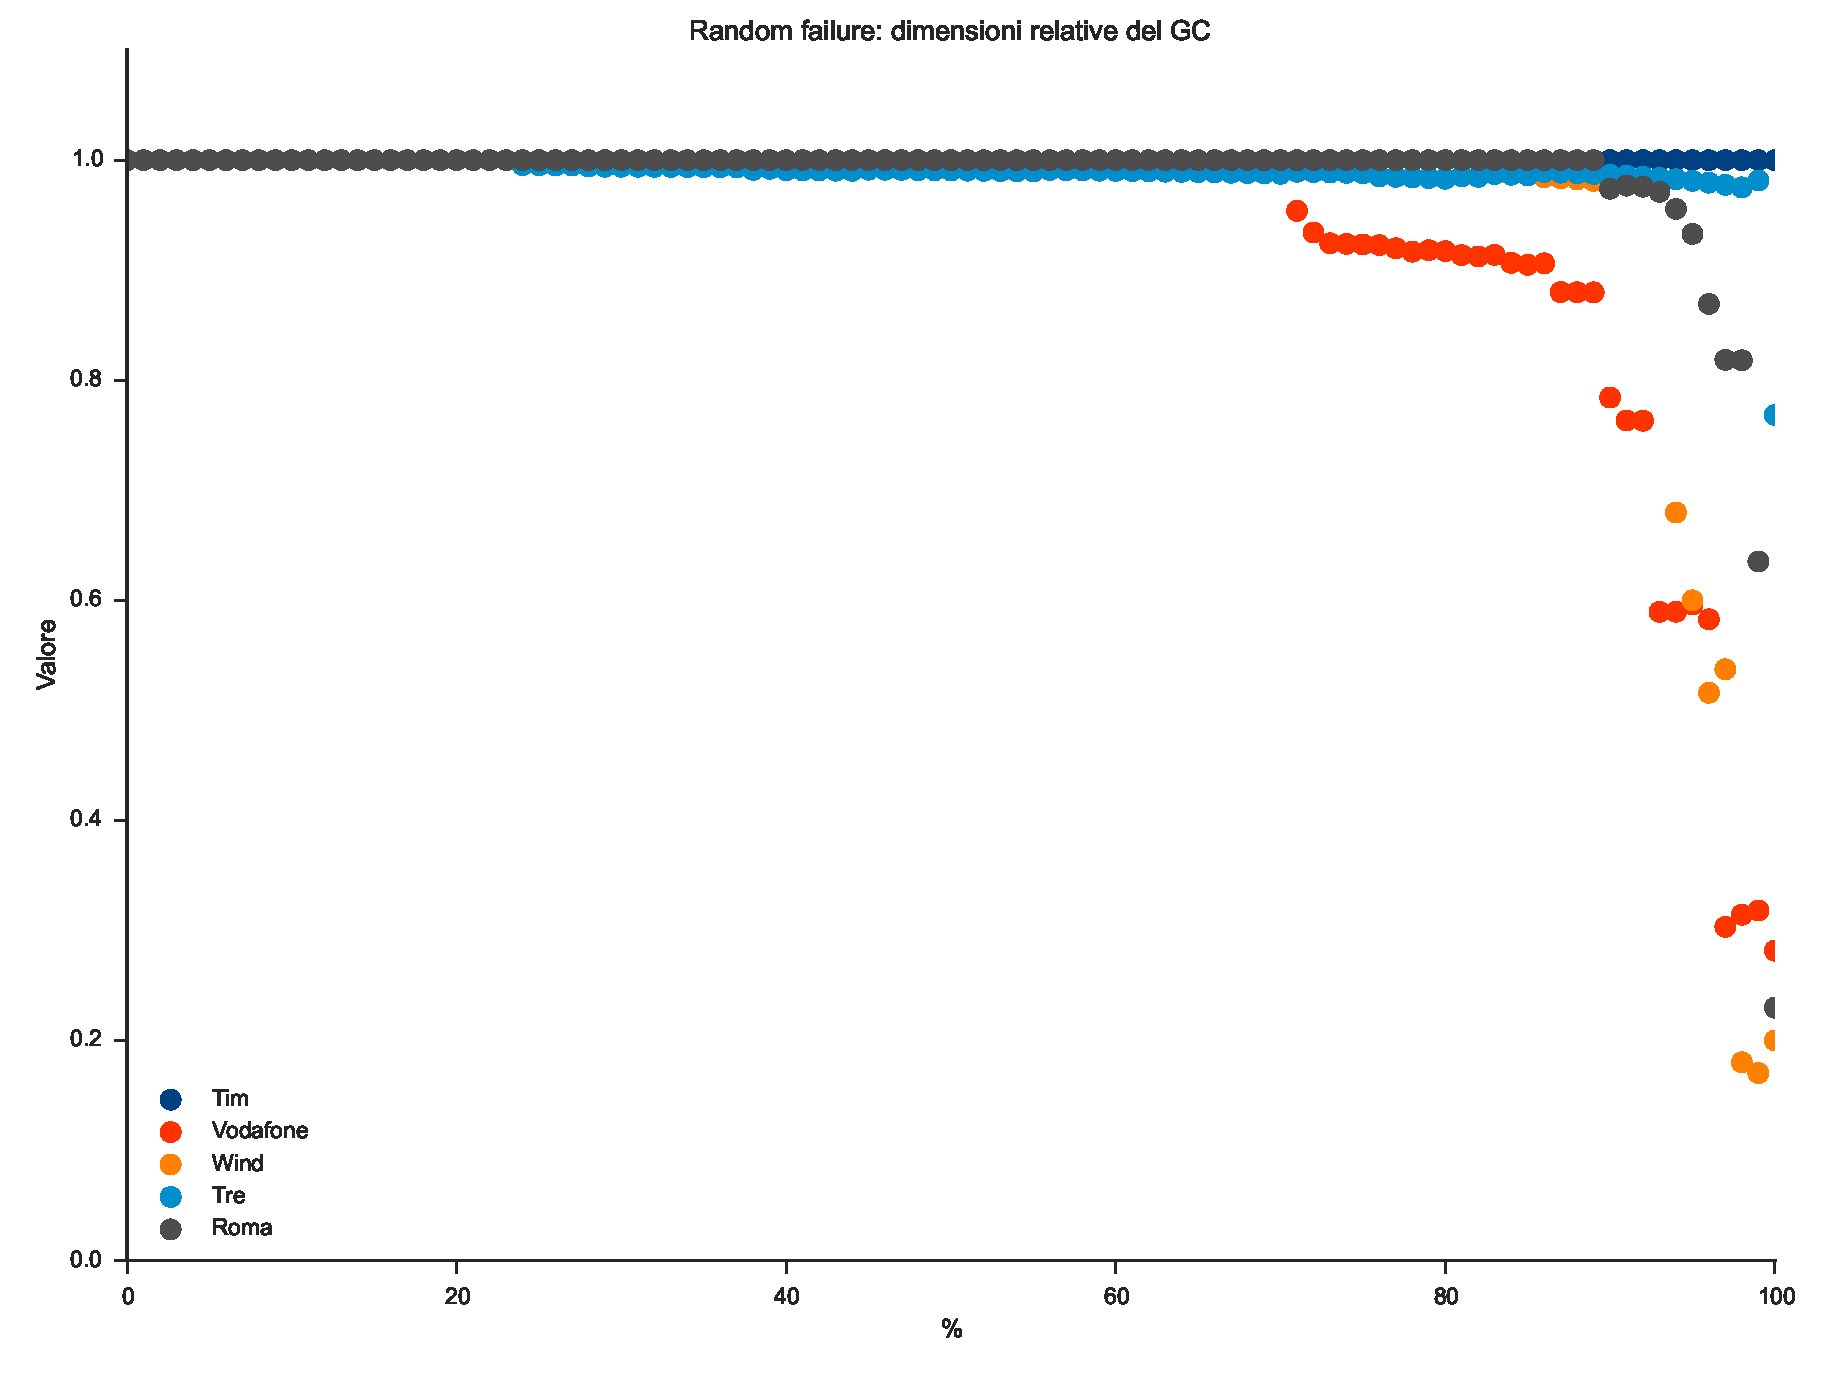
\includegraphics[width=0.47\textwidth]{./Immagini/Attack/gToolFailureGC_Final}}
	$\;$
	\subfloat[$C$]
	{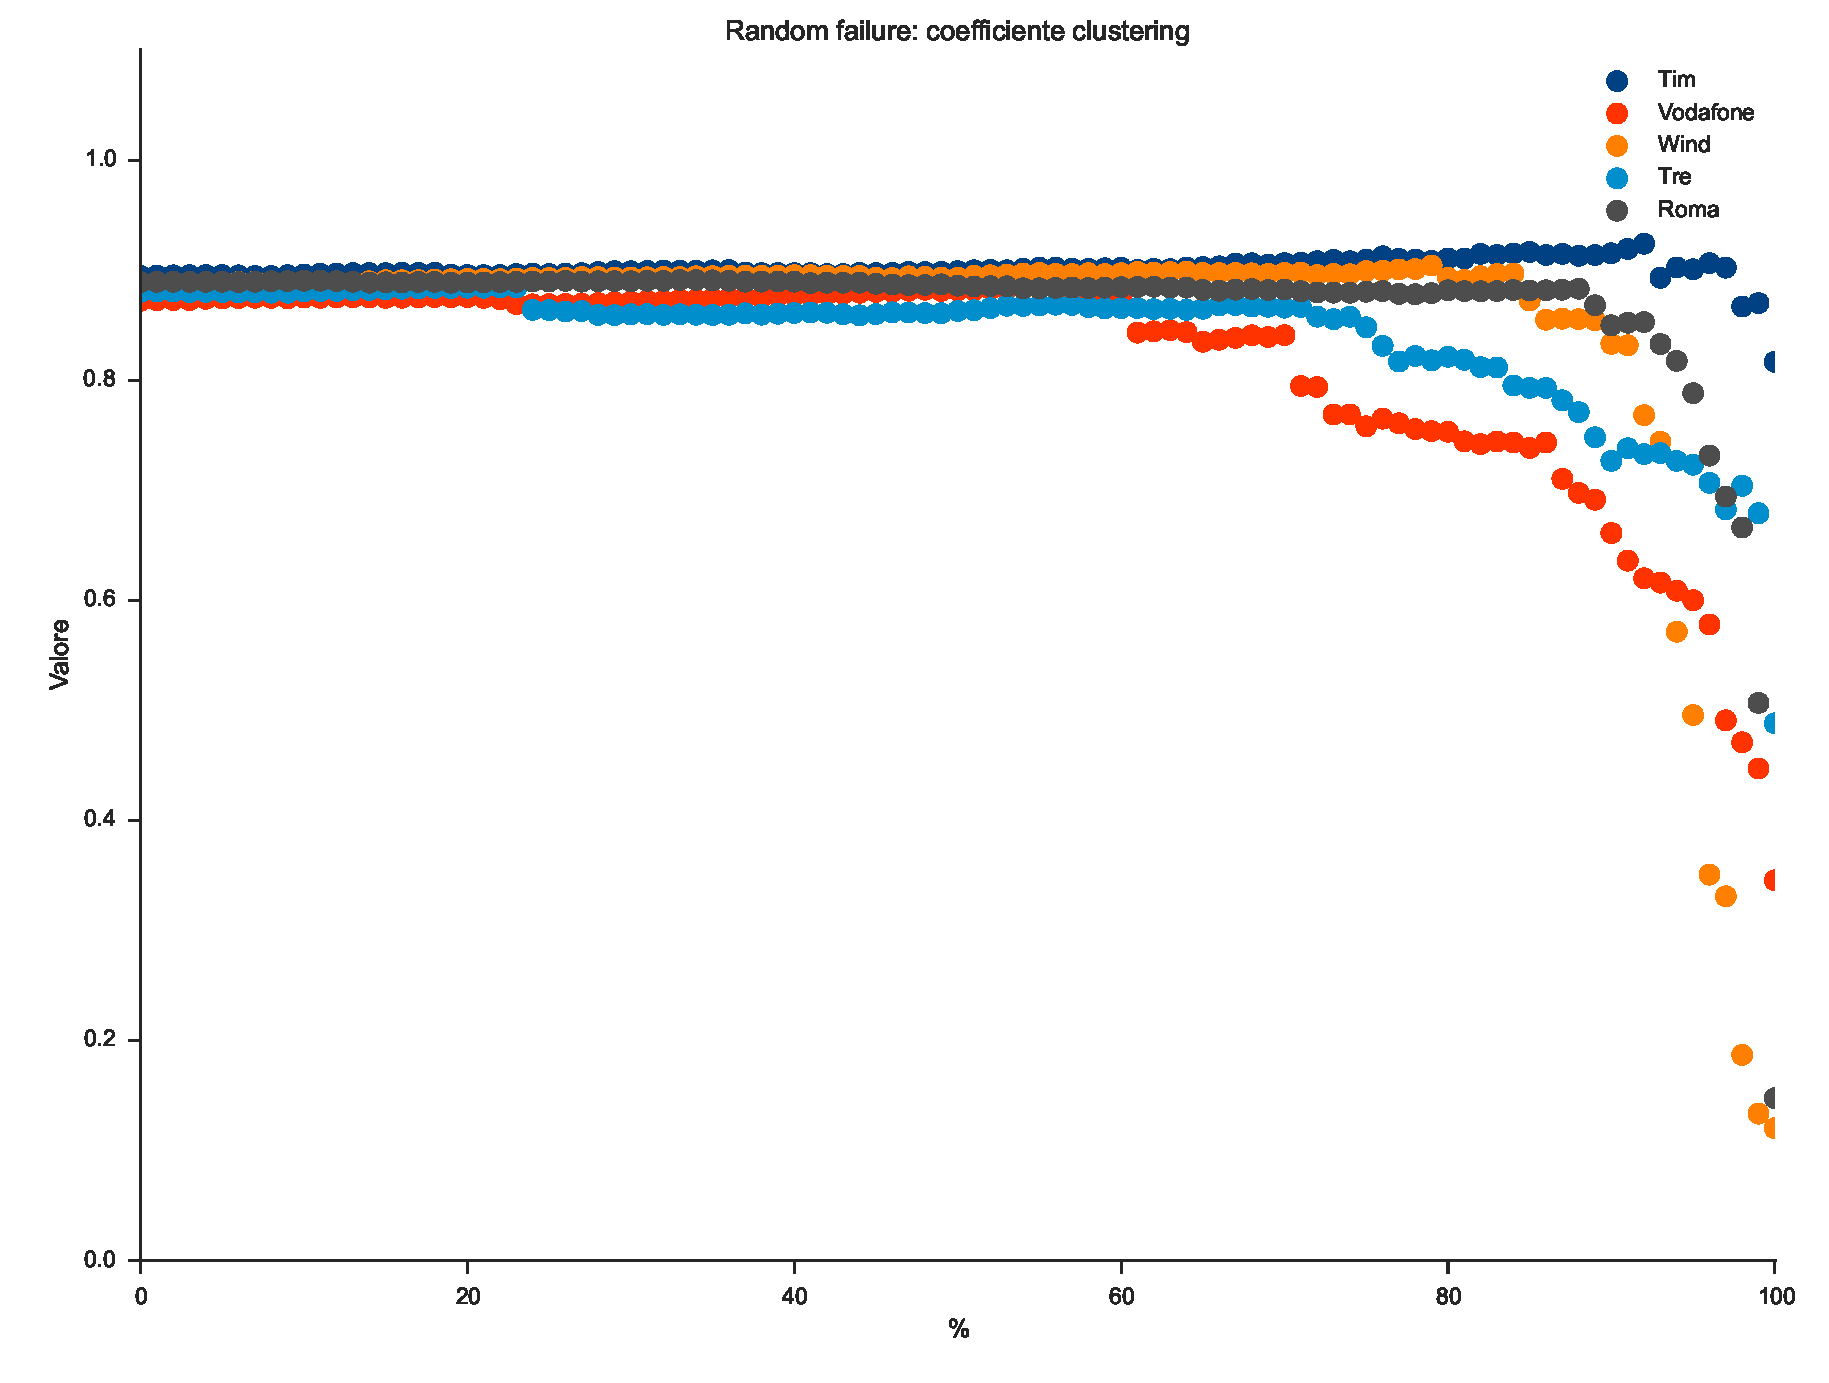
\includegraphics[width=0.47\textwidth]{./Immagini/Attack/gToolFailureC_Final}}
	\\
	\subfloat[$\langle l \rangle$]
	{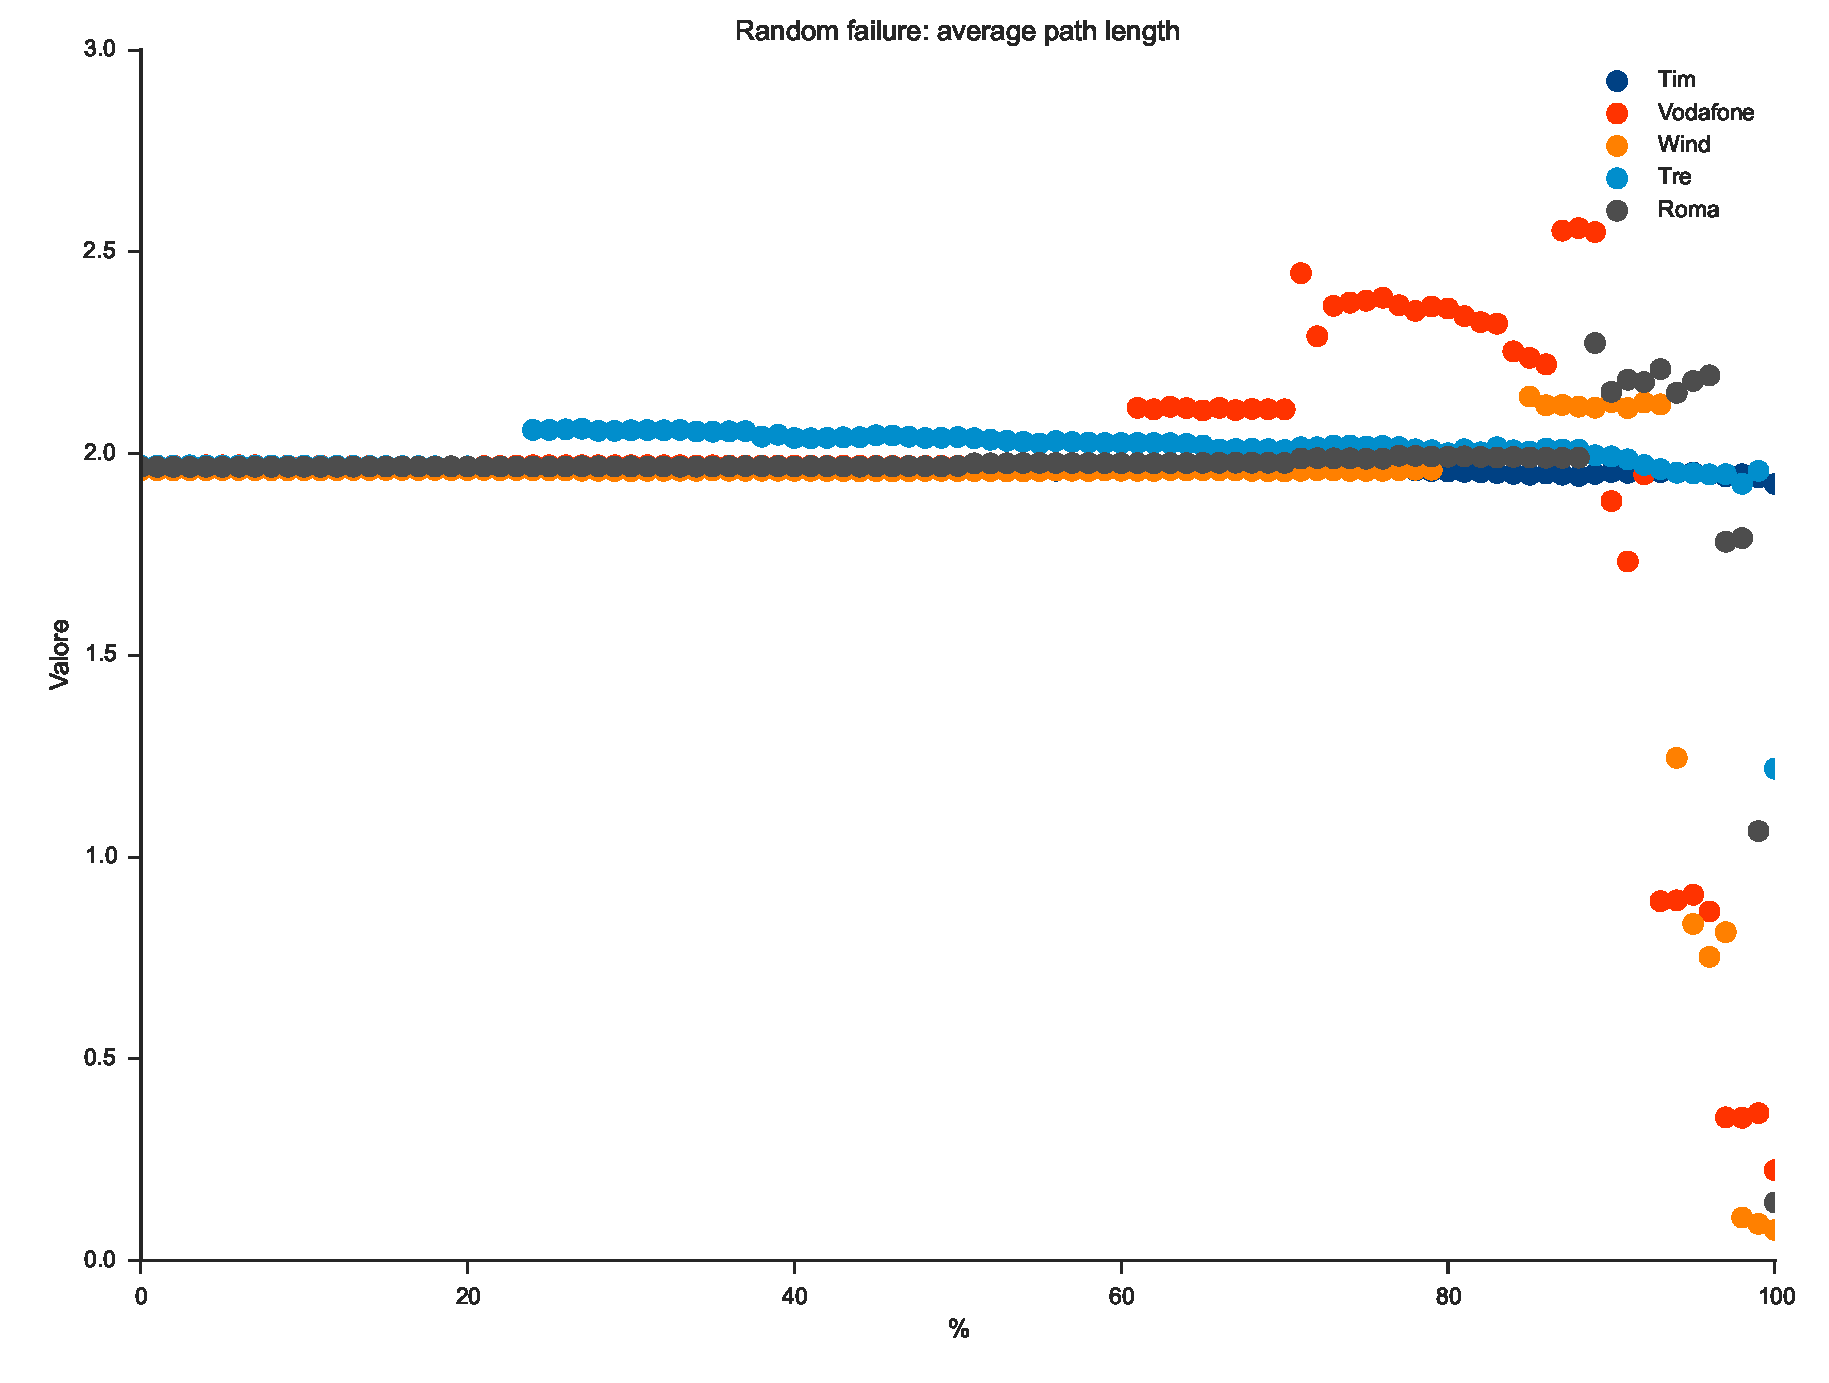
\includegraphics[width=0.47\textwidth]{./Immagini/Attack/gToolFailurel_Final}}
	$\;$
	\subfloat[$D$]
	{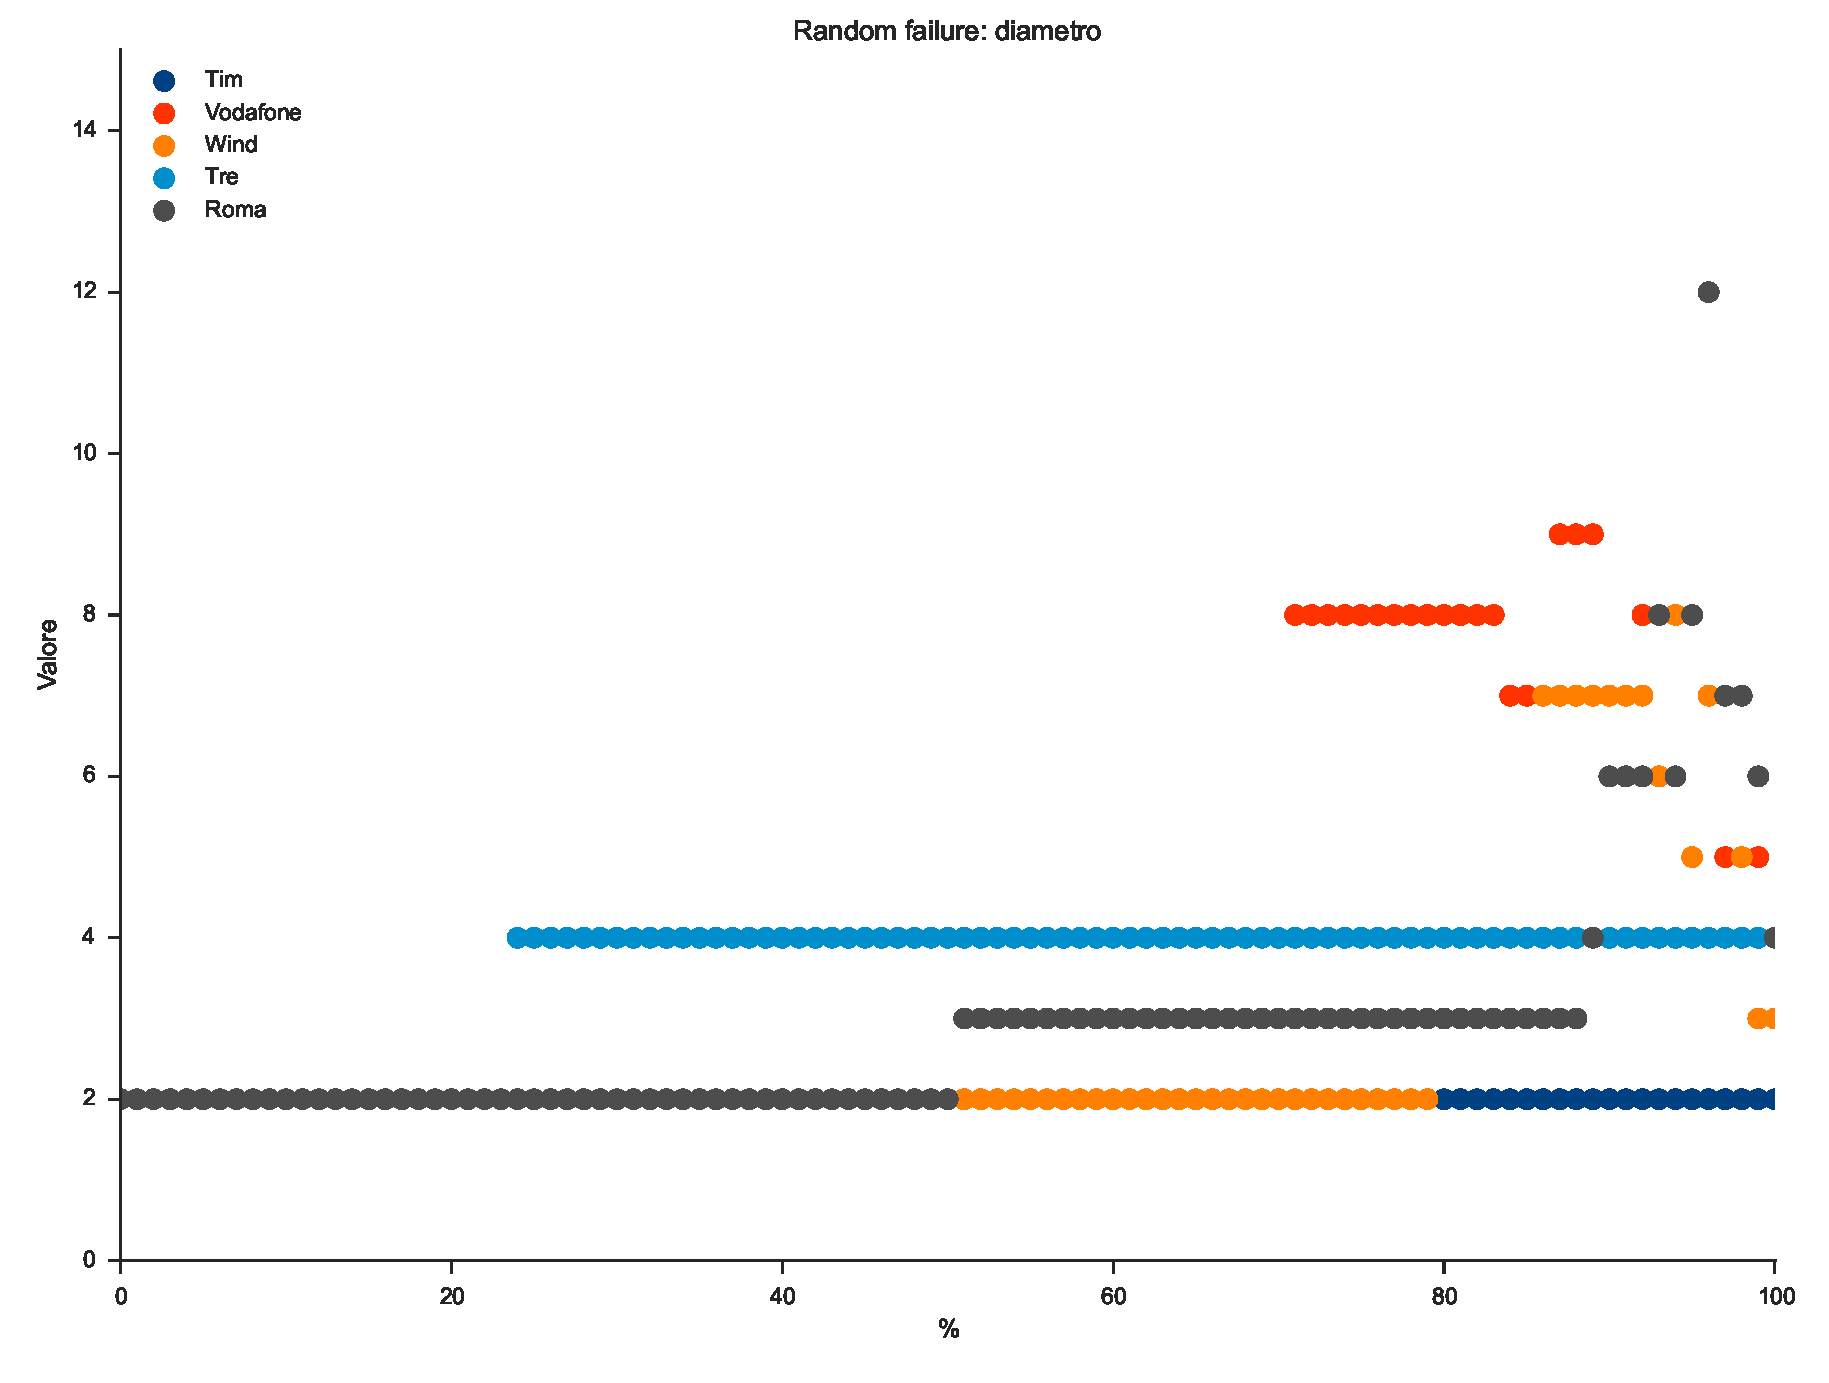
\includegraphics[width=0.47\textwidth]{./Immagini/Attack/gToolFailureD_Final}}
	\\
	\subfloat[$\langle k \rangle$]
	{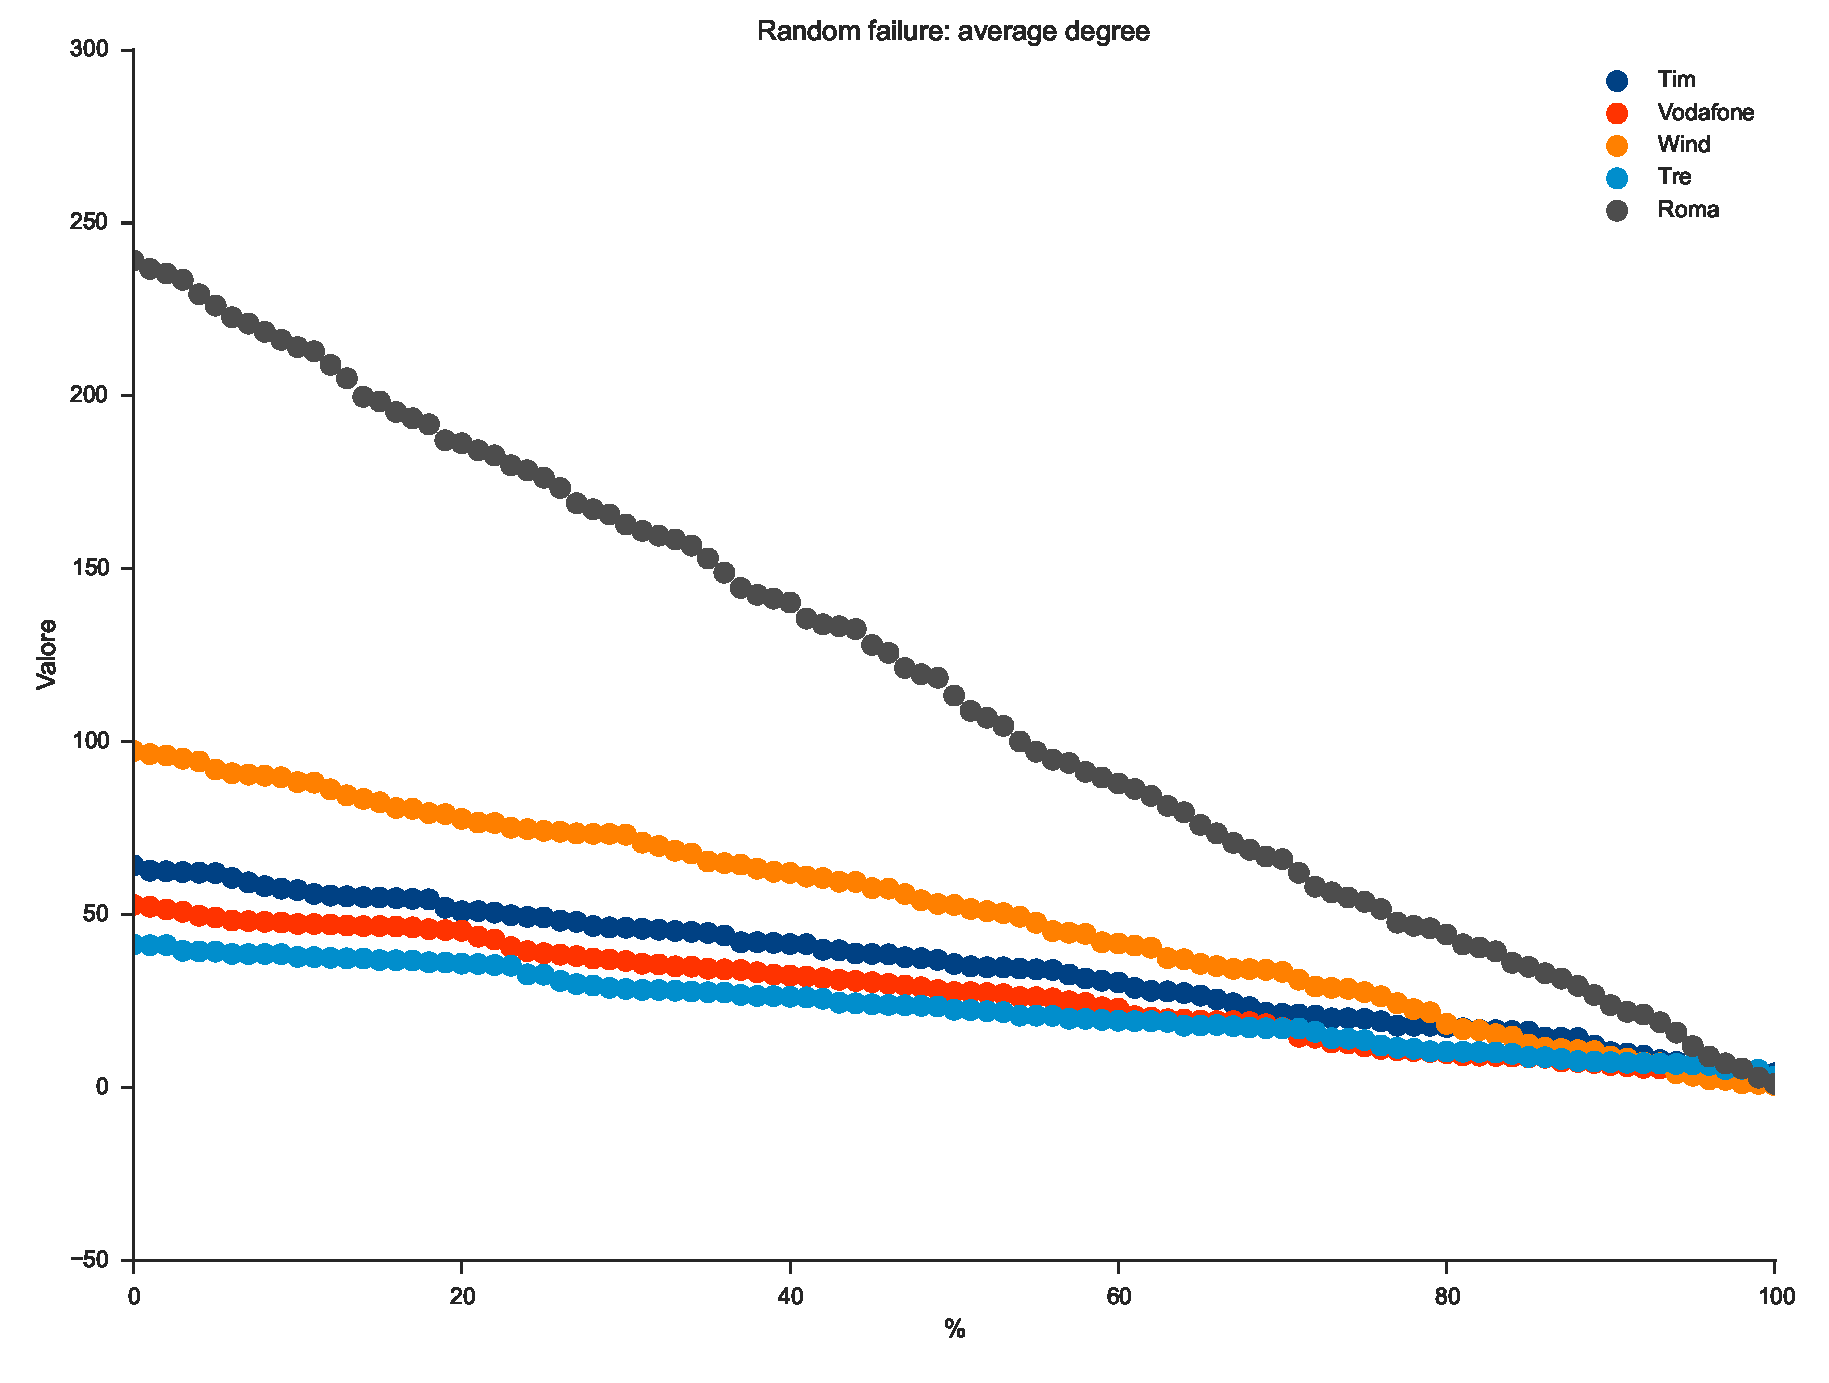
\includegraphics[width=0.47\textwidth]{./Immagini/Attack/gToolFailurek_Final}}
	$\;$
	\subfloat[$\langle k^2 \rangle/\langle k \rangle$]
	{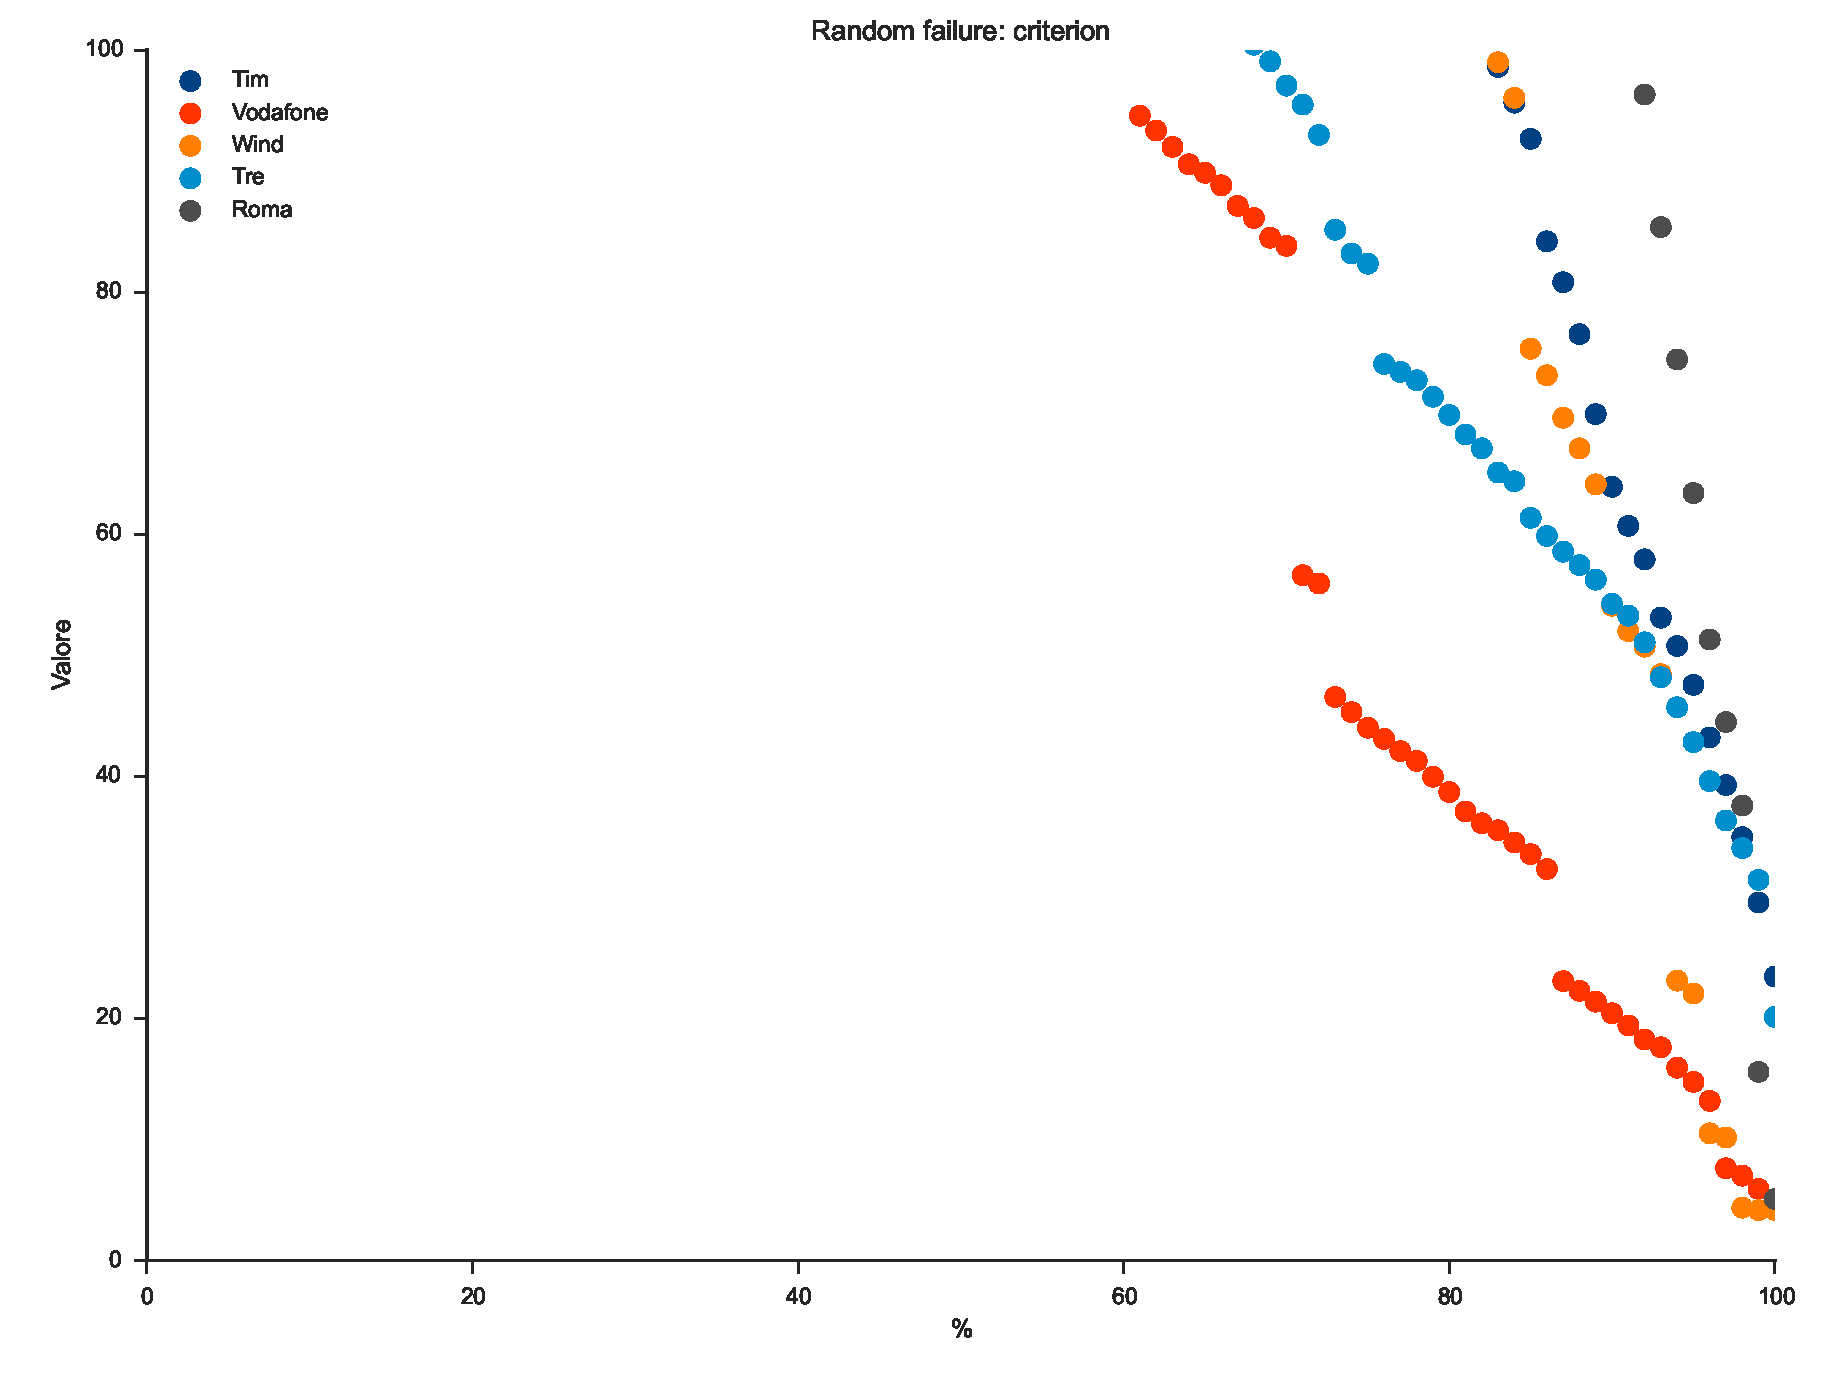
\includegraphics[width=0.47\textwidth]{./Immagini/Attack/gToolFailurec_Final}}
	\caption[Risultati random.]{Risultati per rimozione random}
	\label{fig:fail}
\end{figure}

\begin{figure}[p!]
	\centering
	\subfloat[$GC$]
	{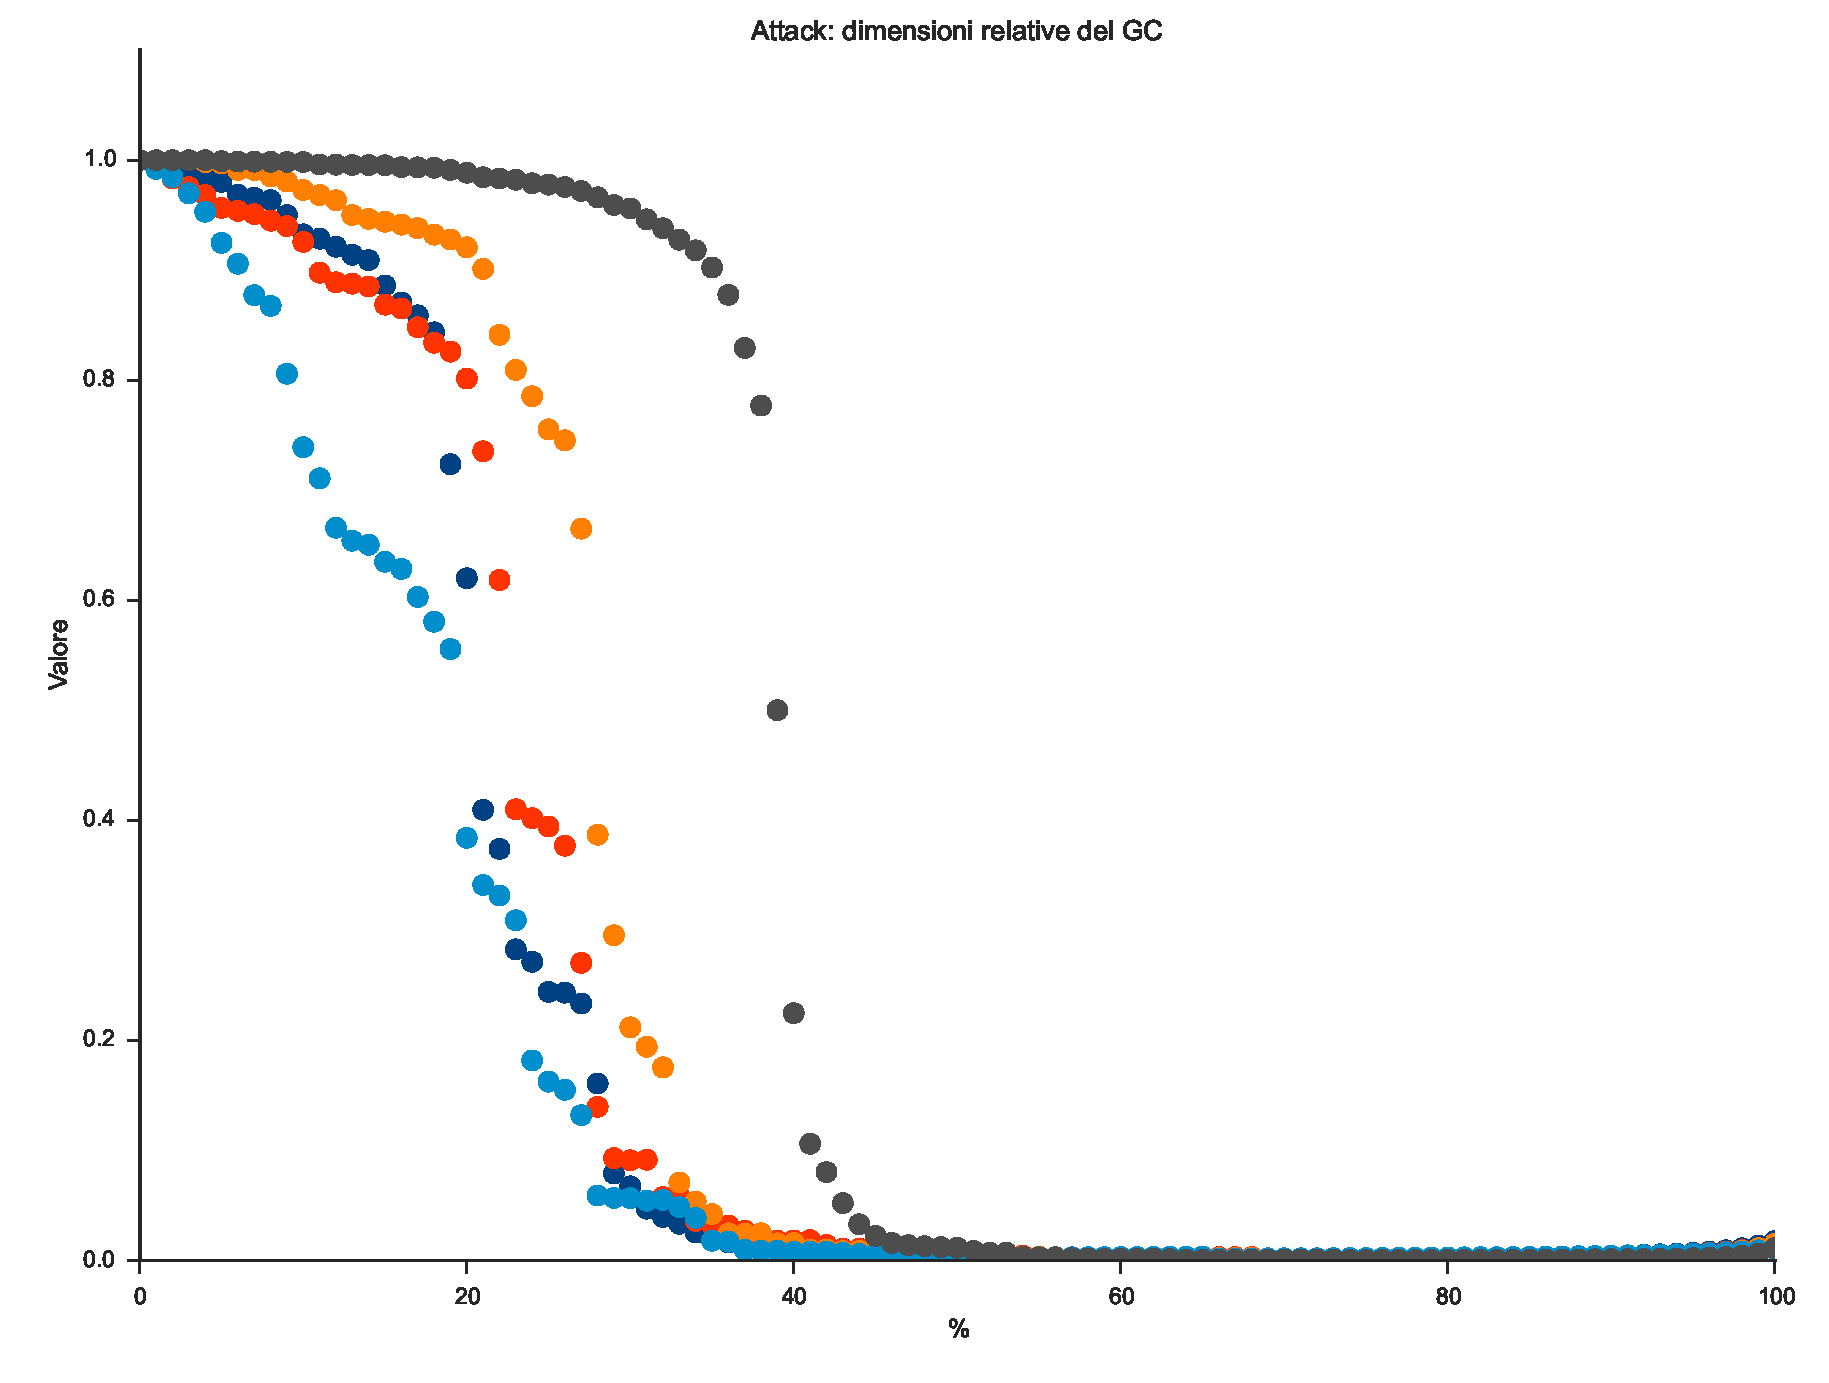
\includegraphics[width=0.47\textwidth]{./Immagini/Attack/gToolAttackGC_Final}}
	$\;$
	\subfloat[$C$]
	{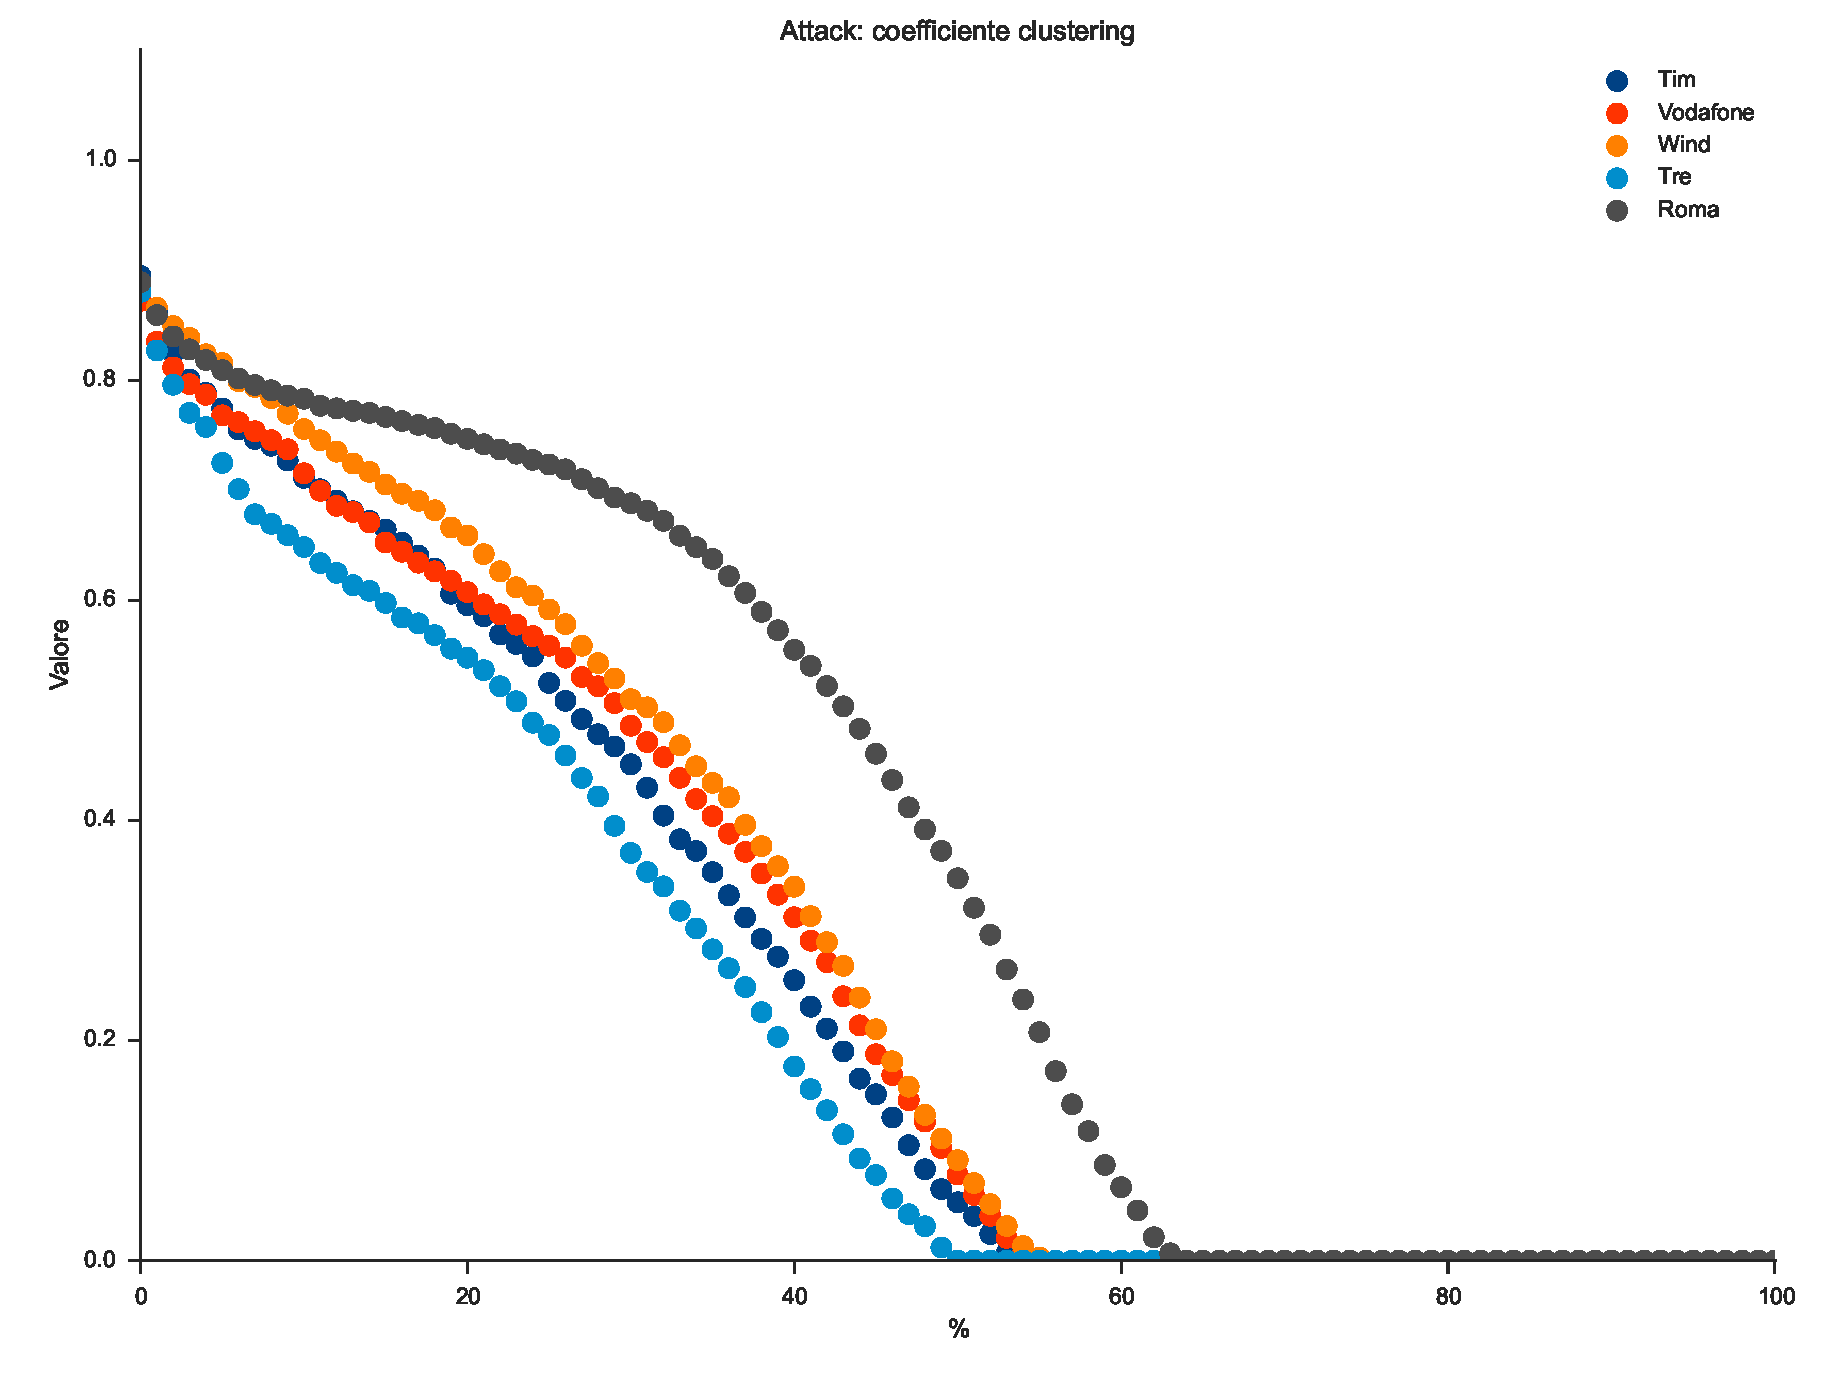
\includegraphics[width=0.47\textwidth]{./Immagini/Attack/gToolAttackC_Final}}
	\\
	\subfloat[$\langle l \rangle$]
	{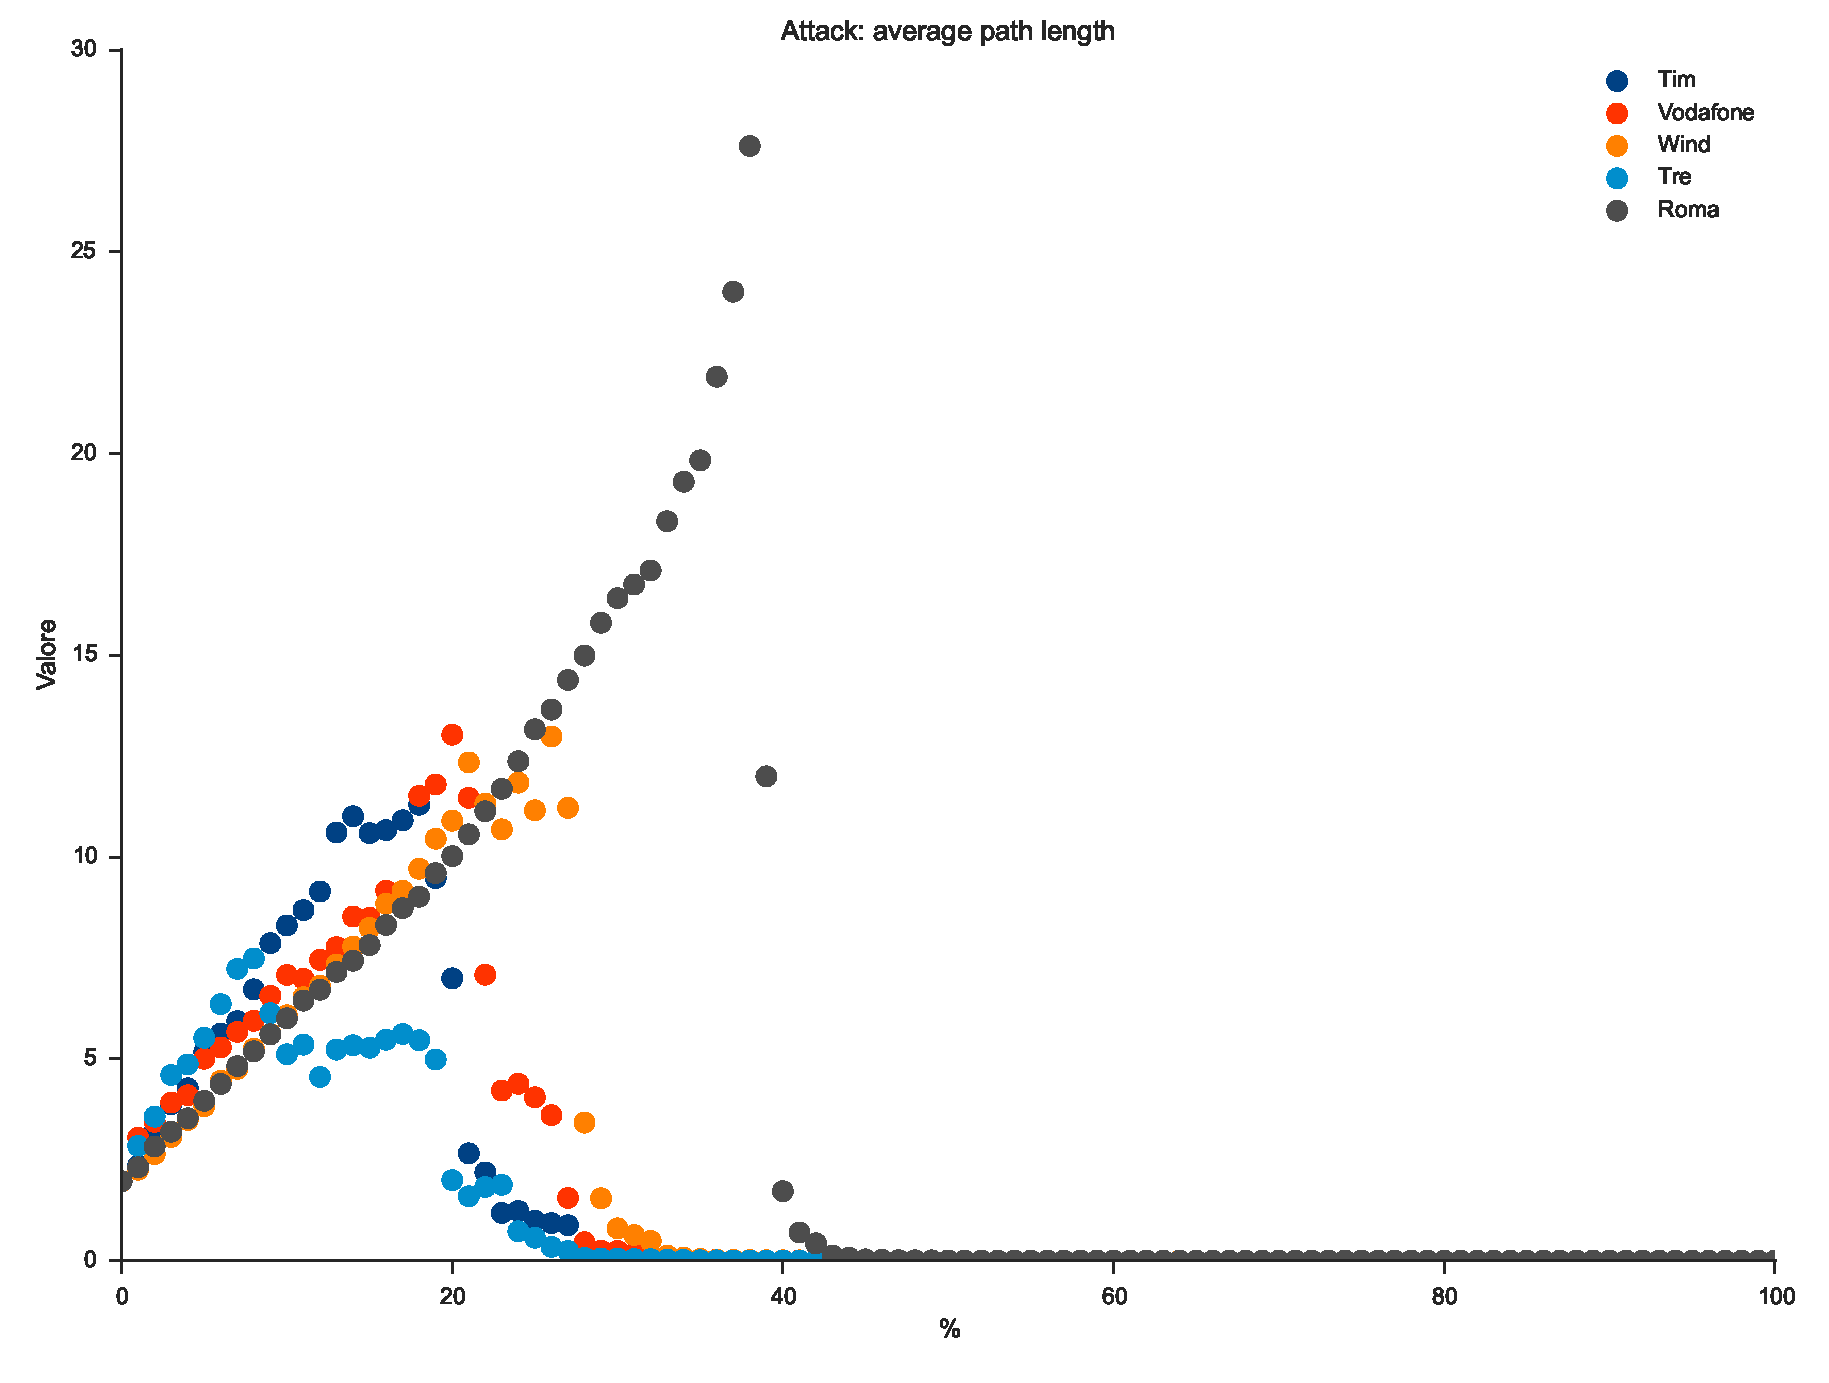
\includegraphics[width=0.47\textwidth]{./Immagini/Attack/gToolAttackl_Final}}
	$\;$
	\subfloat[$D$]
	{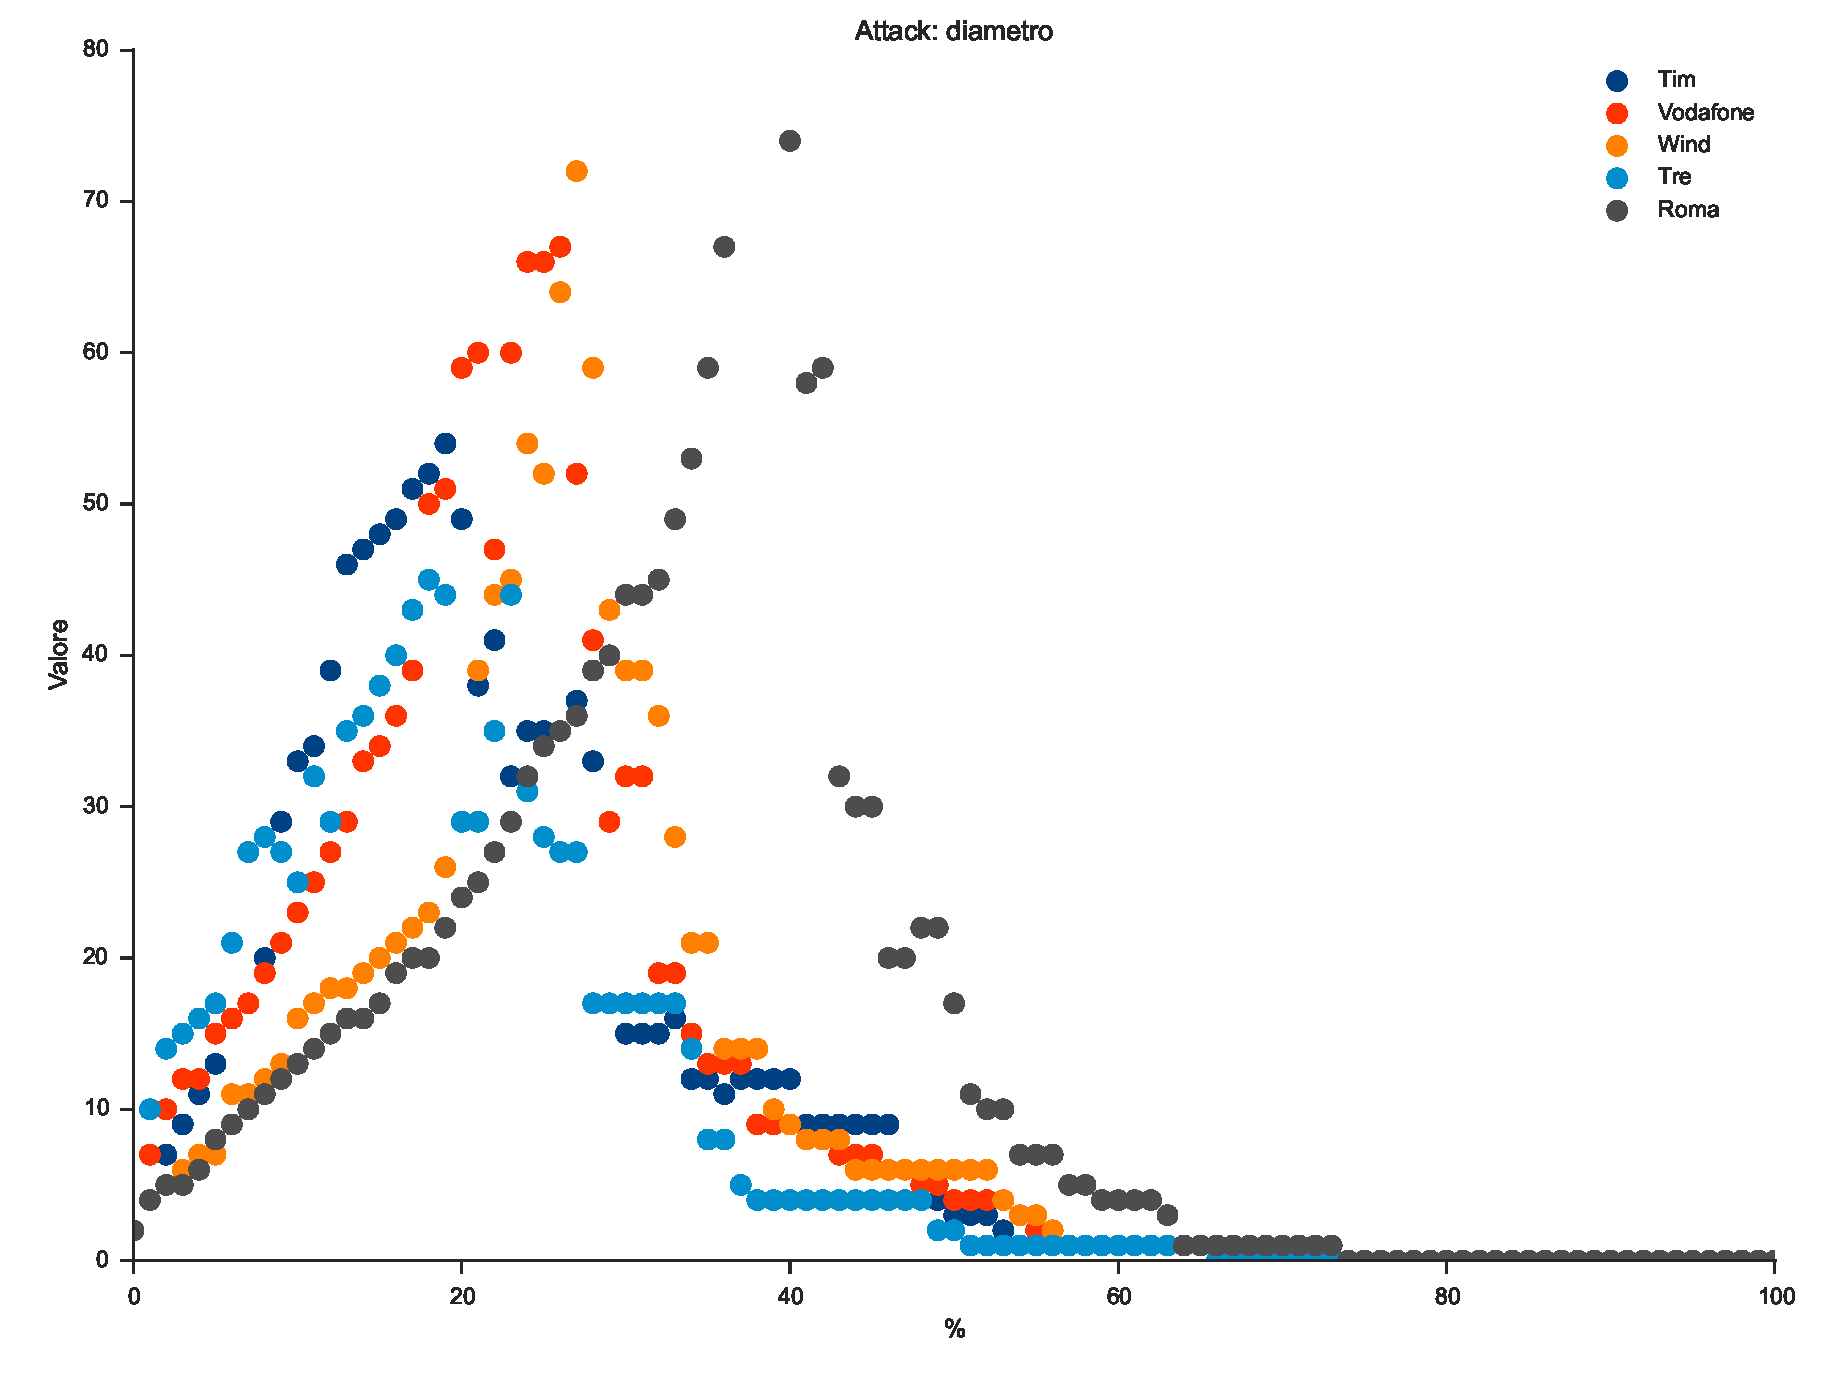
\includegraphics[width=0.47\textwidth]{./Immagini/Attack/gToolAttackD_Final}}
	\\
	\subfloat[$\langle k \rangle$]
	{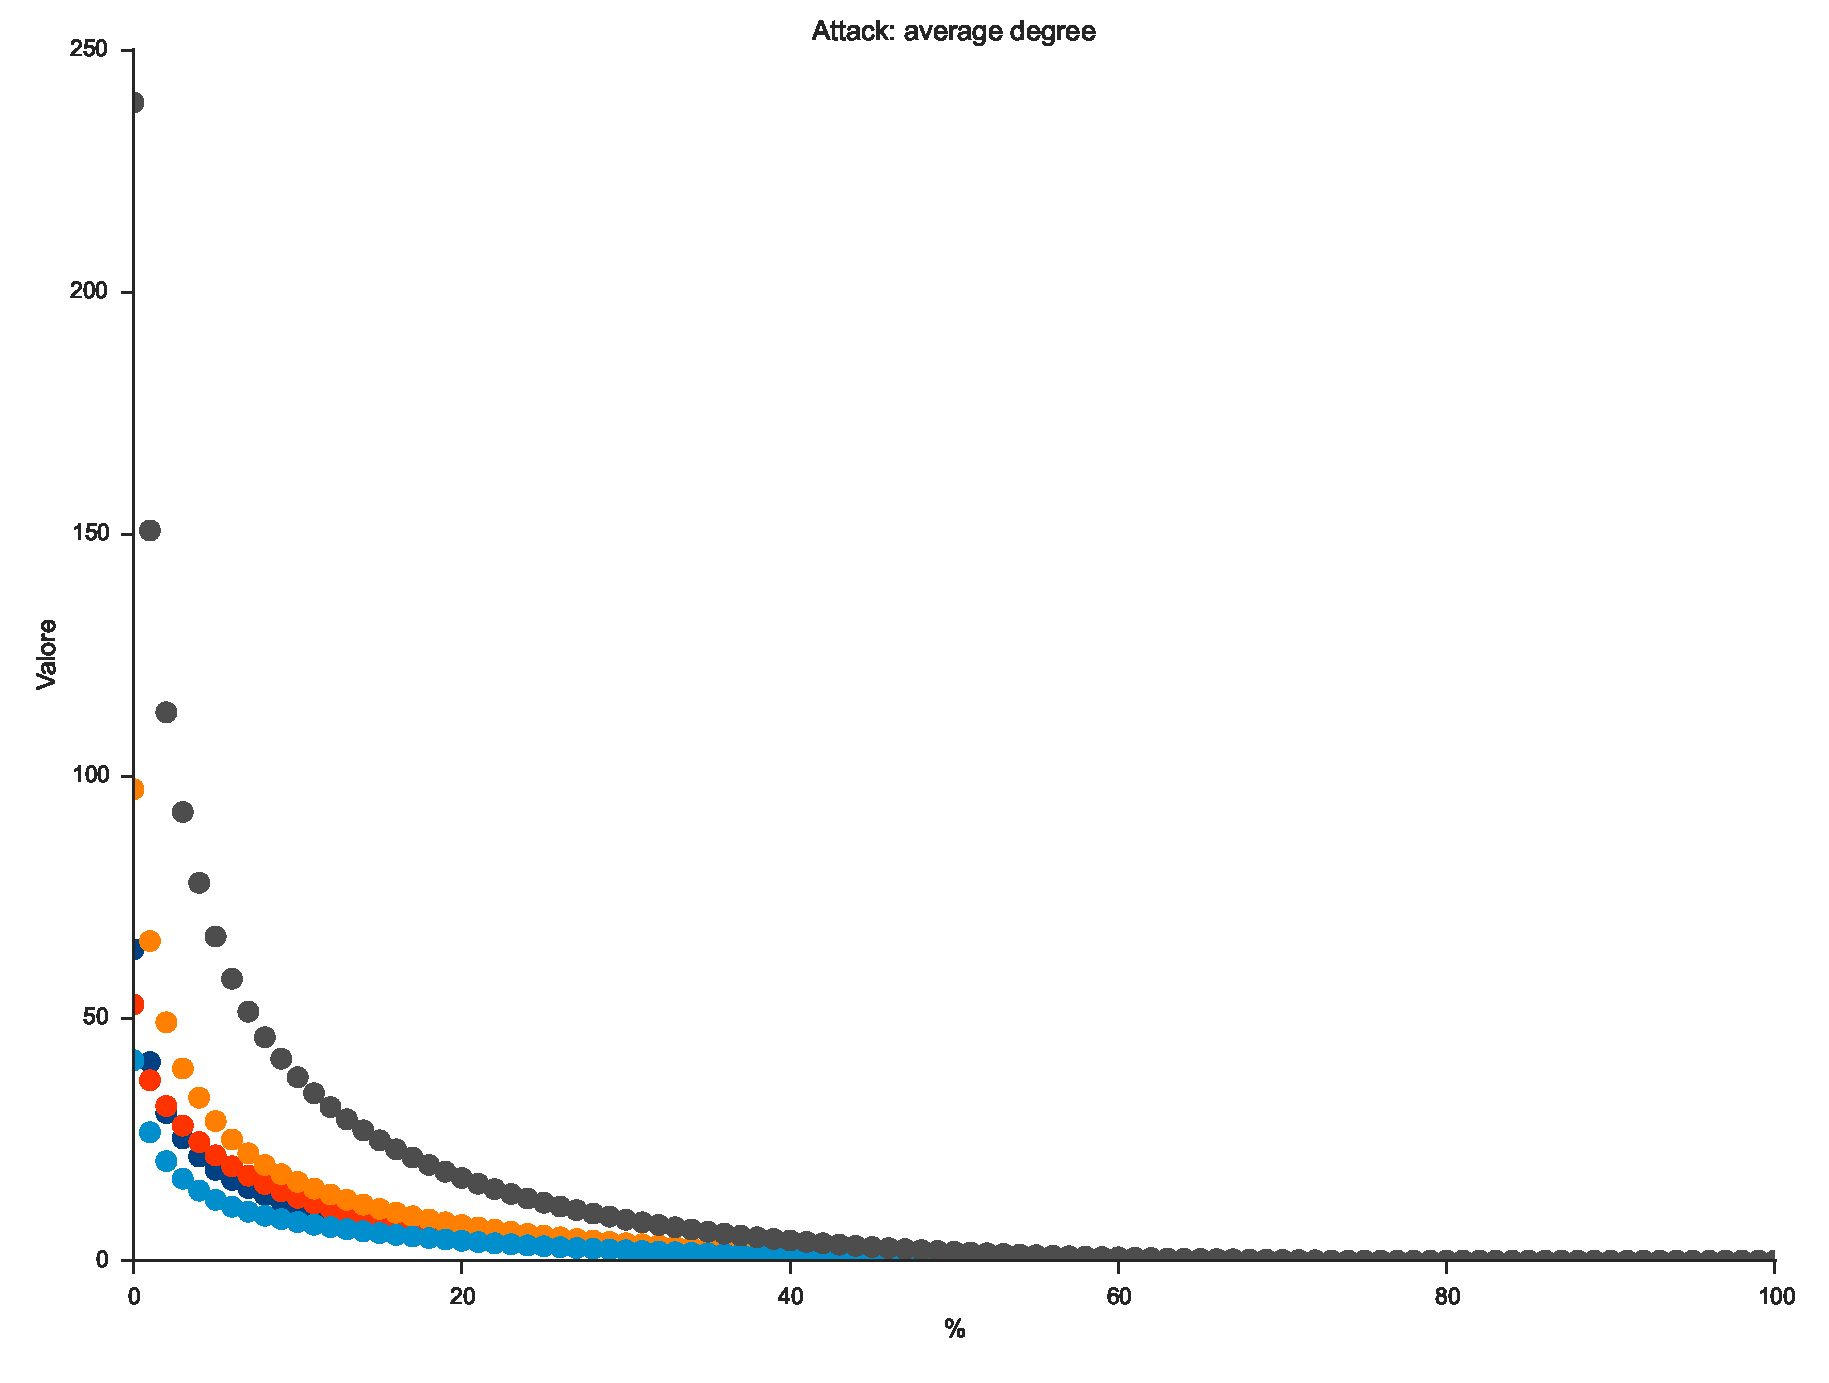
\includegraphics[width=0.47\textwidth]{./Immagini/Attack/gToolAttackk_Final}}
	$\;$
	\subfloat[$\langle k^2 \rangle/\langle k \rangle$]
	{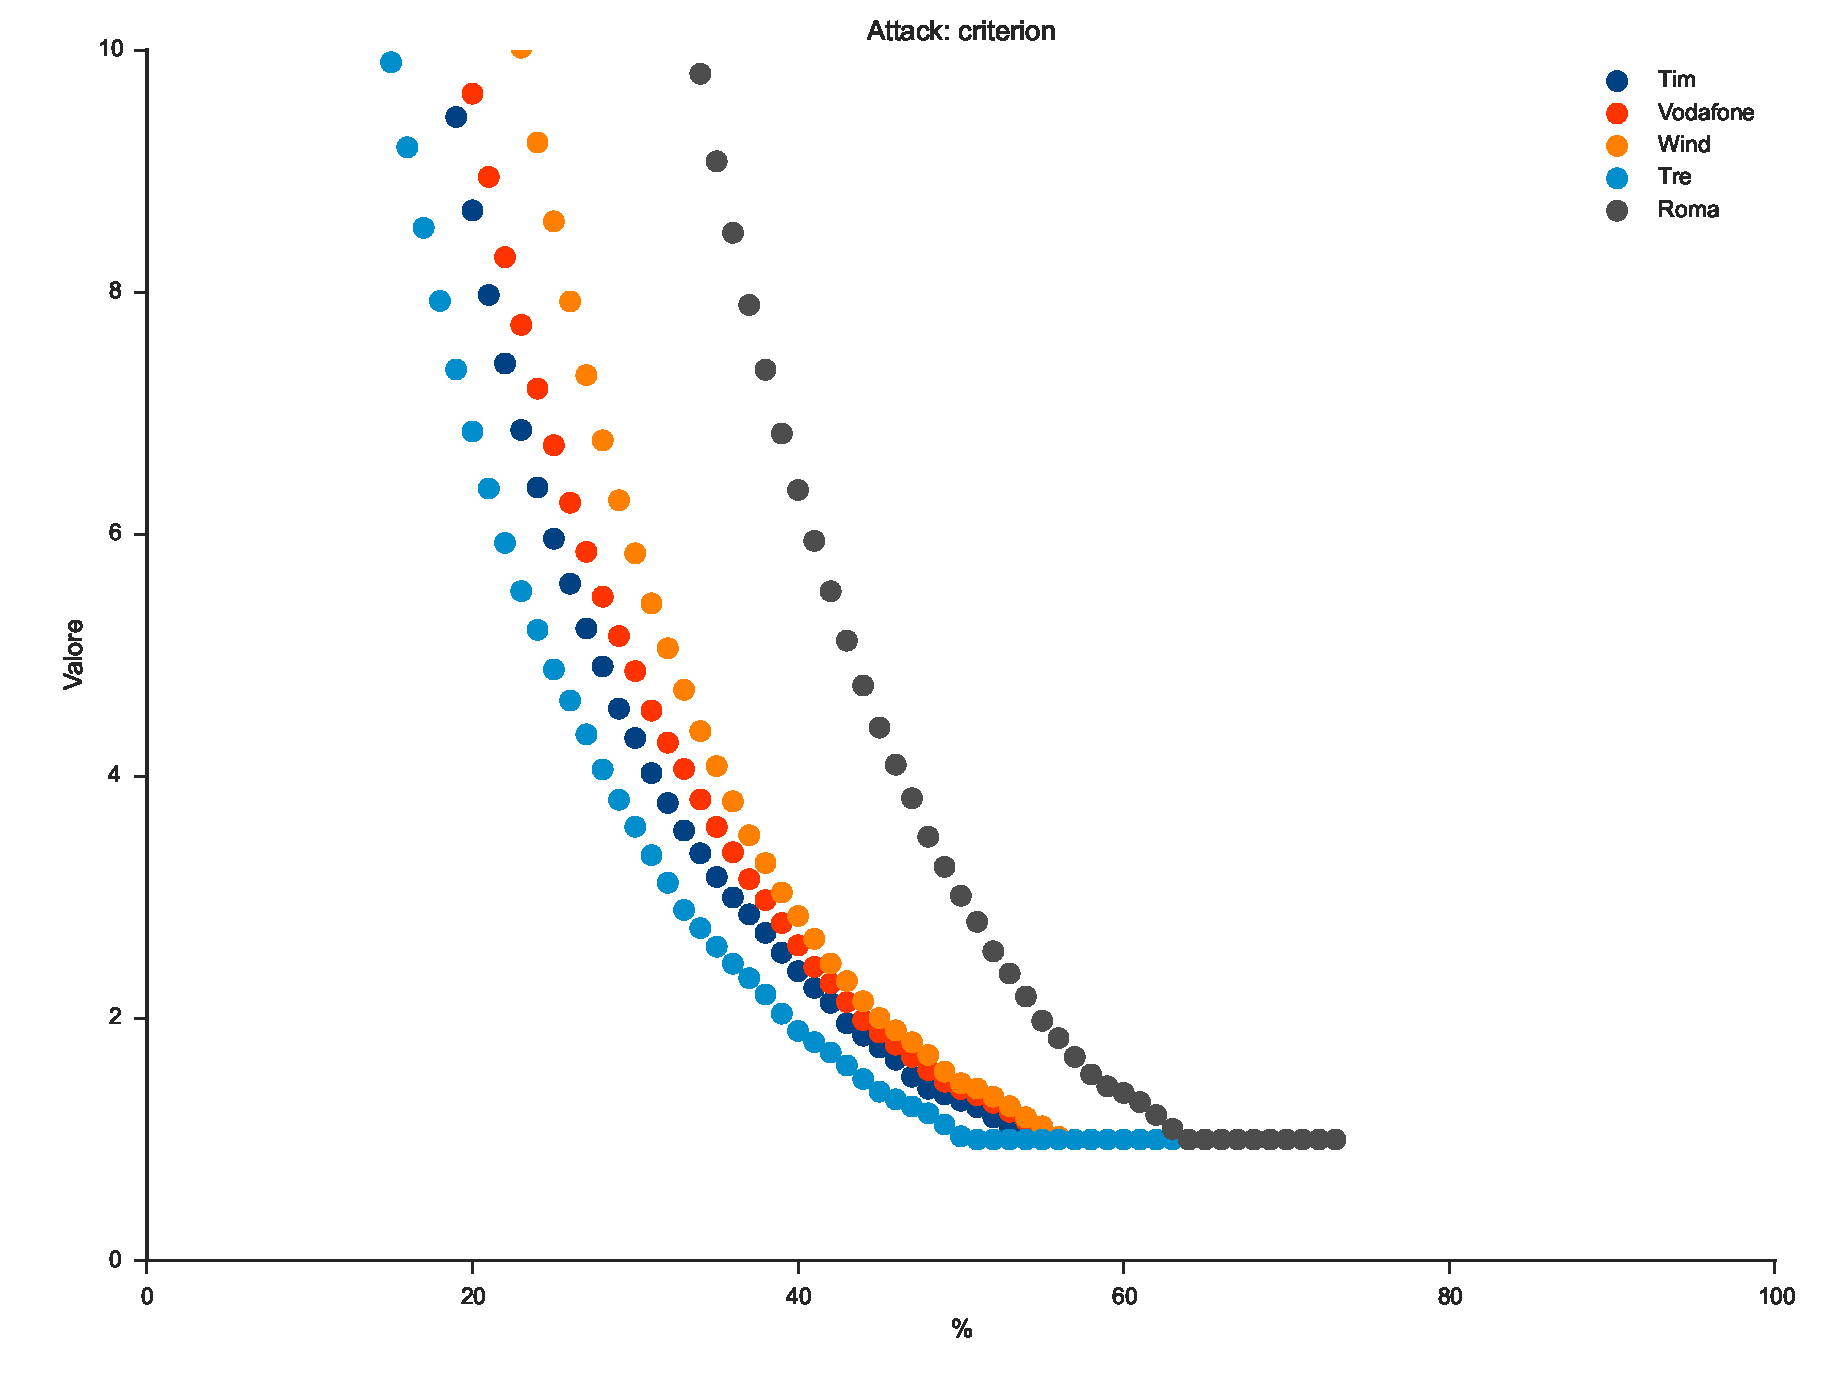
\includegraphics[width=0.47\textwidth]{./Immagini/Attack/gToolAttackc_Final}}
	\caption[Risultati attacco.]{Risultati per rimozione con massima efficienza}
	\label{fig:atak}
\end{figure}
\clearpage
\section{Conclusioni}
Come abbiamo visto, in regime di alta connettività dal punto di vista percolativo si notano poco le differenze tra reti generate secondo un modello scale-free o random. La differenza si nota quando il grado medio della rete è più basso. Per esempio una rete random con $\langle k \rangle \sim 2$ ha $f\sim 50\%$, mentre una rete scale free con stesso $\langle k \rangle$ ha $f\sim 80\%$. Una spiegazione qualitativa sta nel fatto che con una distribuzione del grado a legge di potenza, i nodi meno connessi sono in larga maggioranza, quindi è meno probabile che un attacco random riesca a destrutturare la rete, rispetto a un grafo che abbia una $P(k)$ poissoniana.

Uno studio percolativo su reti reali, quindi, non aiuta a identificare una eventuale invarianza di scala per reti molto grandi e connesse. Tuttavia può essere decisiva per reti più piccole, come piccole comunità, reti locali e alcuni ecosistemi: nonostante la bassa statistica, i comportamento di reti con pochi nodi possono essere distinti in maniera significativa da uno studio percolativo.

Nel caso di reti il cui funzionamento dipende dalla capacità dei nodi di gestire un certo carico, uno studio percolativo dovrebbe anche considerare l'eventualità che con la rimozione di alcuni nodi, altri vadano in sovraccarico e si scolleghino dalla rete, ovvero di un effetto cascata (Motter \citeyear{Motter2002}, Zhao \citeyear{Zhao2004} e \citeyear{Zhao2005}, Wang \citeyear{Wang2009}). È il caso delle reti comunicative, come quelle telefoniche cellulari analizzate o una ipotetica rete mesh costruita con i router WiFi, ma anche ovviamente reti di distribuzioni elettriche, ecc.

Una possibile interessante applicazione dei metodi e degli strumenti usati per analizzare la rete di antenne di Roma potrebbe essere lo studio di città molto più grandi e densamente popolate (come New York o Tokyo), ma servirebbero capacità di calcolo e di memoria molto più grandi di quelle a nostra disposizione. Un altro possibile studio potrebbe essere verificare la possibilità di creare una rete distribuita e aperta con i router WiFi.

%valutare se lasciare o rimuovere
Una rete di questo tipo sarebbe comunque un nuovo concetto di Internet, che potrebbe avere interessanti sviluppi su reti di altro tipo, per esempio sociali, correlate a essa.